% !TEX program = xelatex
\documentclass[11pt]{article}

\usepackage[a4paper,margin=1in,marginparsep=0pt,marginparwidth=0pt]{geometry} %showframe

\usepackage[xetex]{graphicx} % Required for inserting images
\usepackage{eso-pic} %for logos in the background

% fonts
%\usepackage{nunito}
\usepackage{pifont}
 
\usepackage{url}
\usepackage[dutch,english]{babel}

\usepackage{imakeidx} %creating index. it is important to load the imakeidx package before hyperref to make the index pages as links
\usepackage[colorlinks=true,hyperfootnotes=true]{hyperref}
\usepackage{xcolor}
\usepackage{tikz} 
\usepackage{subcaption}

% change predefined section names
\usepackage[nottoc,notlof,notlot]{tocbibind} 
\usepackage[title]{appendix}

\usepackage{tabularray}
\usepackage{caption}
%\usepackage{multirow}
\usepackage{ltablex}
\usepackage{booktabs}

\usepackage{fontspec} %use of custom fonts
\usepackage{enumitem} %itemize list customization

\usepackage{titlesec} %customize look&feel of sections
%\usepackage{tablefootnote}

\usepackage{xesearch} %searching for some terms automatically and highlight
%% define nlesc colors
\definecolor{nlesc-blue}{RGB}{0, 157, 221}
\definecolor{nlesc-purple}{RGB}{53, 6, 57}
\definecolor{nlesc-yellow}{RGB}{255, 178, 19}

%\newcommand{\mythinline}{\noalign{\hrule height 0.8pt}}


%% nlesc logos
\newcommand{\placelogo}[0]{
\AddToShipoutPictureBG{%
%  \AtPageLowerRight{\makebox[1.3\textwidth][r]{%
%    
\includegraphics[scale=1]{img/a0000-img003.jpg}}}}
\AtPageUpperLeft{\raisebox{-8\baselineskip}{\makebox[\paperwidth]{\hspace{16cm}
\includegraphics[scale=1]{img/a0000-img002.png}}}}
  \AtPageLowerLeft{\raisebox{2\baselineskip}{\makebox[\paperwidth]{\hspace{16cm}
\includegraphics[scale=1]{img/a0000-img003.jpg}}}} 
}%
}


%% custom fonts
\defaultfontfeatures{Mapping=tex-text,Scale=MatchLowercase}
\setmainfont[Path = font/, Extension = .ttf,UprightFont = *-Regular, BoldFont = *-Bold, ItalicFont = Nunito-LightItalic, BoldItalicFont = Nunito-Italic]
{Assistant}
%\setmainfont{Assistant}

\parskip=5pt plus 5pt
\parindent=0pt %paragraph space

\setitemize{itemsep=0pt} % linespace in itemized list

%customize look&feel of sections
\titleformat{\section}{\color{nlesc-blue}\fontsize{18}{20}\bfseries}{\color{nlesc-blue}\thesection}{1.5em}{}
\titleformat{\subsection}{\fontsize{16}{18}\bfseries}{\thesubsection}{1.5em}{}
%\titleformat{\section}{\fontsize{11}{15}\bfseries}{\Roman{section}}{1.5em}{USI }

%making links underlined
%\makeatletter
%\Hy@AtBeginDocument{%
%  \def\@pdfborder{0 0 1}% Overrides border definition set with colorlinks=true
%  \def\@pdfborderstyle{/S/U/W 1}% Overrides border style set with colorlinks=true
%                                % Hyperlink border style will be underline of width 1pt
%}
%\makeatother
\hypersetup{linkcolor=nlesc-blue,linkbordercolor=nlesc-blue,urlcolor=nlesc-blue,urlbordercolor=nlesc-blue,citecolor=nlesc-blue}

\newcommand{\status}[1]{\underline{\textbf{#1}}}

\newlength{\myhcolw} %reusable variable for column size
\makeatletter
\let\LT@arraybak\LT@array
\def\LT@array{\setlist[itemize]{leftmargin=*,after=\strut}\LT@arraybak}
\makeatother

% long table style
\UseTblrLibrary{booktabs}

\NewTblrTheme{fancy}{
  \SetTblrStyle{firsthead}{font=\bfseries}
  \SetTblrStyle{firstfoot}{fg=blue2}
  \SetTblrStyle{middlefoot}{\itshape}
  \SetTblrStyle{caption-tag}{red2}
  \setlist[itemize]{leftmargin=*}
}

 \setcounter{footnote}{0}
 
 \newcommand{\ftnotetxt}[2]{
   \footnote{#2\label{#1}}
   }
   
 \newcommand{\ftnotelbl}[1]{
   \textsuperscript{\ref{#1}}
   }


% searching automatically list of special terms, hightlight and add these to the index 
\SearchList{LeadRSEkey}{\colorbox{nlesc-yellow}{#1}\index{#1}}{Lead RSE,LeadRSE} % requires xesearch
\SearchList{PMkey}{\colorbox{nlesc-purple!30}{#1}\index{#1}}{PM}
\SearchList{TLkey}{\colorbox{nlesc-blue!30}{#1}\index{#1}}{TL}
\SearchList{Operkey}{\colorbox{red!20}{#1}\index{#1}}{Finance,Operations,DoO,Controller}

\makeindex   
\usepackage{tablefootnote}




\title{{\fontsize{36}{38}\selectfont \textbf{\color{nlesc-purple}Project Management Protocol of the Netherlands eScience Center}}}
\author{Authors: Netherlands eScience Center Programme Managers}
\date{Date: September 2023\\Version: 2.0}

\begin{document}

\begin{titlepage}

\AddToShipoutPictureBG*{%
  \AtPageLowerLeft{\makebox[1.32\textwidth][r]{%
    
\includegraphics[scale=1]{img/a0000-img001.png}}}}


        \maketitle
        \vspace{8cm}


  
            
\begin{table}[!h]
\resizebox{1.1\textwidth}{!}{%
\begin{tabular}{llc}
\multicolumn{1}{c}{Date} & \multicolumn{1}{c}{version} & Changes   \\
1 October 2023           & 2.0 updates                 & \multicolumn{1}{l}{\begin{tabular}[t]{@{}l@{}}DT and PM mandates, Roles of Directors, PMs role in Ambition 2,\\ SS, KD and external projects, Communications role, Editorial team, \\ breakdown of hours, opportunities beyond project, \\ Technology Status Report, End report\end{tabular}} \\
23 September 2022        & 1.0 initial version         &                                                                                                                                                                                                                                                                                           
\end{tabular}%
}
\end{table}
            
  %      \vspace{0.8cm}




\end{titlepage}

\clearpage
\setcounter{tocdepth}{2}
\tableofcontents

\clearpage
\placelogo{}


\section{Scope and definitions}
\label{sec:scope}

\subsection{Scope}

This document is the official project management protocol for the Netherlands eScience Center. It describes all phases
of a project and the procedures required to successfully complete them.

The scope of this document is the execution of research projects awarded by the eScience Center through calls for
proposals, though other types of projects are also briefly covered. This document gives a detailed description of all
steps, both necessary and optional, that must or may be taken in the execution of projects, reflecting the so-called
\textit{project life cycle}. For each step, the document indicates the responsibilities of the project team members
(RSEs) and other eScience Center employees (e.g. Programme Managers, Finances, Directors Team) involved in the
process.

Call procedures follow a separate protocol~\cite{call-protocol-2015} and are
not covered by this document. The call procedure protocol ends with the formal awarding of projects by the eScience
Center Governing Board or the Directors Team (DT), the notification of Lead Applicants and the formalization of the
awarding by means of a \textit{toekenningsbrief} ('Awarding letter’). The
current document describes all activities that (need to) take place from that moment onwards, until the formal closing
of the project. An independent evaluation of projects, including impact, output, process and collaboration with project
partners is outside of the scope of the current document, and will be published as a separate document or a subsequent
version of this document in the future. 

This document has been approved by the DT and will be subject to evaluation and possible adaptation annually.

The structure of this document largely follows the project life cycle (see Section~\ref{sec:scope:lifecycle}); the
protocol describes activities in chronological order.

\subsection{Stakeholders}
An eScience project is a project involving the eScience Center, where responsibility is shared between different
stakeholders who each have their own roles and responsibilities during specific phases of the project.


%\resizebox{\textwidth}{!}{%
%\begin{tabular}{p{0.15\textwidth}p{0.15\textwidth}p{0.2\textwidth}p{0.2\textwidth}p{0.1\textwidth}}
\begin{tabularx}{\linewidth}{p{0.12\textwidth}|p{0.12\textwidth}|p{0.12\textwidth}|p{0.25\textwidth}|p{0.25\textwidth}}
\toprule
\textbf{Stakeholder} & \textbf{Abbreviation} & \textbf{Assignment}& \textbf{Role}& \textbf{More info}\\
\midrule
\endfirsthead
\toprule
\textbf{Stakeholder} & \textbf{Abbreviation} & \textbf{Assignment}& \textbf{Role}& \textbf{More info}\\
\toprule
\endhead
\midrule
\multicolumn{5}{r}{}
\endfoot
\bottomrule
\endlastfoot  
Lead Applicant & LA & main applicant and recipient of the grant & primary contact for the eScience Center project, accountable for the (quality of the) scientific contribution to the project & responsibilities defined in the call text, the Terms and Conditions document, and potentially a Consortium/Collaboration agreement.  \\\hline
Programme Manager                                  & PM                    & assigned by the PM team~\footnote{All PMs, led by the Programme Director, constitute the PM team.}                                                                                          & accountable for the eScience contribution to a project, responsible for realization of project results given predetermined resources and timelines, project budget holder                                                              & Full text of responsibilities available in the PM job profile document (see Section 5 for the reference) and PM mandate (Appendix~\ref{app:pm-mandate}) \\\hline
Lead Research Software Engineer                    & Lead RSE              & appointed by accountable PM                                                                                       & responsible for the timely execution of the project, main contact person for the project with other stakeholders                                                                                                                       & More details on responsibilities, see the formal role description of Lead RSE (Appendix~\ref{app:leadRSE}).                                          \\\hline
Research Software Engineer (assigned to a project) & RSE                   & assigned by the accountable PM                                                                                    & responsible for the timely completion of the project                                                                                                                                                                                   & All RSE activities coordinated by Lead RSE in agreement with PM.                                                                     \\\hline
Consulting Research Software Engineer              & Consulting RSE        & involved at request of Lead RSE or accountable PM                                                                 & responsible for contributing expertise to a project for a limited but predetermined time, can be involved in some of the key meetings, in addition to an expertise contribution                                                        & All activities coordinated by Lead RSE in agreement with PM in case the project team needs additional expertise.                     \\\hline
Technology Lead                                    & TL                    & assigned by the TL team~\footnote{All TLs, led by Director of Technology, constitute the TL team.}                                                                                          & acts as point of contact for Lead RSE to the TL team. Safeguards the technological aspects of a project; accountable for the quality, reuse and sustainability of the research software developed.                                     & The TLs team is responsible for internal training programme of RSEs.                                                                 \\\hline
Section Head                                       & SH                    & assigned by the PM/SH team~\footnote{All SHs, led by Executive Director, constitute the SH team.}                                                                                       & line manager of RSEs, responsible for monitoring the overall effectiveness of RSEs in bringing projects to completion; maintain overview of a research domain.                                                                         & The SH team assigns one SH to each RSE team, and the SH ensures that team keeps its capacity and planning up to date.                \\\hline
Communications                                     &                       &                                                                                                                   & advise and facilitate internal and external communications of projects, including but not limited to showcasing projects through news items, website, newsletters, social media, interviews and videos.                                &                                                                                                                                      \\\hline
Community Manager                                  & CM                    &                                                                                                                   & advise on developing outreach activities and promoting community engagement, responsible for external training programme                                                                                                               &                                                                                                                                      \\\hline
Secretary                                          &                       &                                                                                                                   & organizes formal meetings, provide with agenda and slide template, invitation text, list of participants (with emails), and timeline.                                                                                                  &  \href{mailto:secretaries@esciencecenter.nl}{secretaries@esciencecenter.nl}                                                                                         \\\hline
Programme Director                                 & PD                    &                                                                                                                   & the escalation point for PMs, the contact point of PMs to DT for project related changes that need the DT decision, approves the workshops plans (in the agreement with F\&C on the financial part). The budget holder of Acquisition. &                                                                                                                                      \\\hline
Director of Technology                             & DoT                   &                                                                                                                   & The escalation point for TLs, the contact point of TLs to DT, accountable (and responsible) for licences and Intellectual Property (IP), software sustainability budgets holder                                                        &                                                                                                                                      \\\hline
Director of Operations                             & DoO                   &                                                                                                                   & handles legal questions (e.g., contracts, Collaborative Agreements and guest agreements)                                                                                               &                                                                                                                                      \\\hline
Finance \& Control                                 & F\&C                  & part of Operations, includes Controller, and led by DoO                                                           & responsible for maintaining financial project administration in Exact                                                                                                                                                                  & \href{mailto:finance@esciencecenter.nl}{finance@esciencecenter.nl}                                                                                            \\\hline
Directors Team                                     & DT                    & comprised of DoT, DoO, General Director and PD                                                                    & approves formal decisions regarding projects (e.g., budget changes)                                                                                                                                                                    &                                                                                                                                      \\\hline
GDPR contact person                                &                       & appointed by the DT, see the intranet for contact information                                                     & consults on GDPR~\cite{GDPR} or privacy-related issues in the project                                                                                                                                                                             & The eScience Center has not appointed a Data Protection Officer. GDPR aspects must be discussed with the contact person.             \\\hline
eScience Center project team                       & eScience project team & comprises RSEs, PM and TL working on the project                                                                  & responsible for the timely completion of the project                                                                                                                                                                                   &                                                                                                                                      \\\hline
Project team                                       &                       & comprises the eScience project team, LA and their team (including team members indicated in the project proposal) & responsible for the timely completion of the project                                                                                                                                                                                   &                                                                                                                                      \\\hline
Editorial Team                                     &                       &                                                                                                                   & provides support with outreach                                                                                                                                                                                                         & The eScience Center maintains a blog, and has presence in major social networks                                                     
%\end{tabular}%
%}
\end{tabularx}


\subsection{Types of projects}
The eScience Center receives an annual budget from NWO and SURF, the larger part of which is allocated to projects
submitted by researchers working at eligible research performing organizations in the Netherlands in the form of the
in-kind provision of RSEs. Projects may also be funded from external sources (henceforth referred to as \textit{an
external project) }or funded from the annual budget but carried out internally.

By awarding subsidy to a project or by pledging a contribution to an external project, the eScience Center takes on the
obligation to deliver high-quality work in a timely manner.

\subsubsection{Call projects}
The eScience Center publishes a range of calls. Each project is a part of a specific call (regular calls such as
OEC/ASDI, CIT/DTEC/eTEC/JEDS, SSI, or calls in collaboration with other funders such as ADAH, Big Data \& Health, GO,
JCER, eTEC-BIG, ESI-FAR). Projects from the regular calls before 2021 are partly in-cash, while projects awarded later
are fully in-kind (plus a reserved budget for workshops).

Calls can reserve part of the project or the call budget to serve the eScience Center agenda to increase the impact of
software beyond the project itself. Henceforth this will be referred to as the software sustainability budget, formerly
known as generalization budget). The budget is intended for software generalization, reuse and sustainability, and
community building. The DoT is the holder of this budget. Details concerning this budget are included in the Awarding
letter. See Section~\ref{sec:opportunities:ss} for more information.

Project teams (mainly Lead RSE, PM and TL) are expected to consult the specific call text, Awarding letter
(‘Toekenningsbrief’), Terms and Conditions document (‘Bijzondere voorwaarden’, ‘Subsidieregeling’, etc.), Consortium/Collaboration Agreement (CA), and/or
contracts for grant terms and conditions. The LA is responsible for adhering to the conditions of the project, while
the PM, with the help of the Lead RSE, monitors this.

In our call projects, most of the total requested budget is dedicated to project work and project-related activities.
The remaining part (referred to as “general activities”) covers activities that benefit our ability to contribute to
high-quality research, such as the professional development of RSEs through training, work meetings, conferences, etc,
as well as the administrative coordination and project management within the eScience Center. It is up to the PMs and
RSEs in consultation with the SHs to fairly distribute hours for general activities across all the projects they
contribute to (cf. Section~\ref{sec:exec:budget}). The exact percentage set aside for general activities is defined in
the call within which a project has been awarded.

\subsubsection{External projects}
Projects funded externally by e.g. NWO or the EU, or via private-public partnerships, are governed by external funding
conditions specified in a contract or agreement that may supersede our own rules. The budgets of these projects need to
be approved by F\&C and the DoO. Again, the project team (mostly, Lead RSE, PM, TL) must consult the specific call
text, Awarding letter, Terms and Conditions document, Consortium/Collaboration Agreements, contracts for the conditions
and rules. The LA is responsible for adherence to the rules and conditions, while the PM with the help of the Lead RSE
monitors this. Projects under external funding are covered partially by this protocol.\footnote{A budget for writing
grant proposals for external funding, use of it follows the process described in “External funding” (see Section
\ref{sec:opportunities:external-funding} for more information).}

\subsubsection{Other projects}
This document only briefly covers other types of projects such as those funded through Ambition 2, namely Dissemination
\& Community (D\&C), Knowledge \& Development (KD)\footnote{cf. Netherlands eScience Center strategy~\cite{nlesc-strategy} to get familiar with the term.} and Fellowship projects in 
Section~\ref{sec:opportunities:fellowship} and Appendix~\ref{app:pm-role}.

\clearpage
\subsection{Project life cycle overview}
\label{sec:scope:lifecycle}

\begin{figure}[!h]
    \centering
    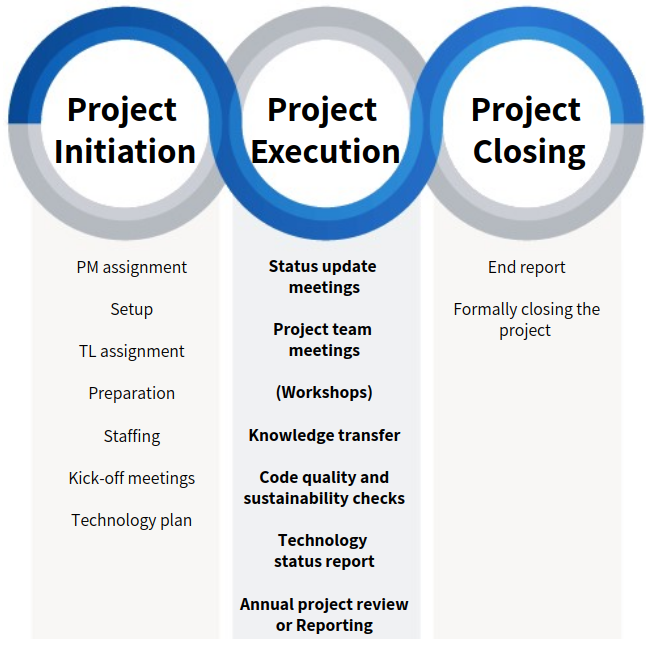
\includegraphics[scale=0.5]{img/lifecycle-stages.png}
    \caption{Project lifecycle stages}
    \label{fig:project-lifecycle}
\end{figure}

At the eScience Center, a standard project life cycle is a three-phase process (see Figure~\ref{fig:project-lifecycle}). First, project stakeholders initiate the
project. Next, the project team executes the project and monitors its progress. Finally, once the project reaches its
end, it is formally closed.

These three phases are covered in detail in the next sections.

\clearpage

\section{Project Initiation}
\label{sec:init}
The project initiation phase starts immediately after the project has been granted. Its goal is to set up the project
within the eScience Center, including a planning in terms of staffing and a work plan.

For \textbf{external projects} and projects from specific calls (e.g., collaborative calls), Finance ensures that all
paperwork is in place (e.g., contracts, Consortium/Collaborative Agreements, Memorandum of Understanding) before making
a project active in Exact, allowing RSEs to write hours spent on the project. The PD regularly keeps PMs up to date on
outstanding applications for external funding, signals to PMs and Finance whenever a project has been granted, and hands
over relevant documents (such as proposal, agreements made, preliminary budget, etc) to PMs. 

PMs are accountable for call projects. For the \textbf{external projects}, PMs assign a PM and Lead RSE to the project
(i.e., the RSE involved in the submission procedure). Together with the Lead RSE the PM works with the project partners
to get all paperwork in order (such as a subcontract), see Section~\ref{sec:init:legal}. 

\subsection{PM assignment}
Each project has one accountable PM. The PM team assigns PMs to new projects at the first PM meeting following the
granting decision, records the assignation and asks Finance to update Exact with new budget holder information (the newly
assigned PM). If agreement over an assignment is not reached, the PD makes the final decision in their capacity as PM
team chair.

Should the accountable PM become unavailable for an extended period, the PM team can decide to put another PM in charge
of the project.

\textbf{Responsible: PM team.}

\subsection{Administrative Setup}
The table offers an overview of the responsibilities of the different stakeholders in setting up a project:

\begin{longtblr}[
  theme = fancy
  %
]{
  colspec={|p{0.15\textwidth}|p{0.15\textwidth}|p{0.65\textwidth}|}, width = 1\linewidth,
  rowhead = 1, %rowfoot = 1,
  row{1} = {font=\bfseries},
  column{1} = {font=\bfseries},
  row{odd} = {white}, row{even} = {white},
  row{1} = {gray!20}, %row{Z} = {nlesc-yellow},
  cell{4}{1} = {r=2}{t},
}
\toprule
    What & By & Responsible for  \\  
\toprule
    Exact  & Finance  &
    \begin{minipage}[t]{1\linewidth}
    \begin{itemize}\itemsep0em
        \item Creating project code
        \item Entering and uploading attachments
        \item Making PM budget holder 
    \end{itemize} 
    \end{minipage}  \\
  \midrule
    Project portfolio on SharePoint~\cite{proj-portfolio}  & Finance  & 
    \begin{minipage}[t]{1\linewidth}
    \begin{itemize}\itemsep0em
        \item Creating folder in project portfolio (with template subfolder \& documents)
        \item Uploading granting package documents (incl. Awarding letter), signed start form, CA if applicable
    \end{itemize} 
    \end{minipage}  \\
  \midrule  
    Research Software Directory (RSD), project page and software pages & PM  & 
    \begin{minipage}[t]{1\linewidth}
    \begin{itemize}\itemsep0em
        \item Creating an RSD project page~\cite{rsd-nlesc}, putting placeholder image with the eScience logo\ftnotelbl{ft:logo}.
        \item Signalling requirements for corporate website to Communications 
        \item Copying website summary from the proposal (if applicable) or writing a summary and obtaining approval from LA for edited versions  
        \item Finding appropriate image (e.g., royalty-free images offered by shutterstock.com and unsplash.com) 
        \item Ensuring Lead RSE has a maintainer access to the RSD page
    \end{itemize} 
    \end{minipage}  \\
 \midrule
      & Communications & 
    \begin{minipage}[t]{1\linewidth}
    \begin{itemize}\itemsep0em    
       \item Advising and reviewing content for the pages, including editing summaries, supporting with images 
    \end{itemize} 
    \end{minipage}  \\
  \midrule
    Corporate website  & Communications &  
    \begin{minipage}[t]{1\linewidth}
        \begin{itemize}\itemsep0em
            \item Ensuring content is displayed on the corporate web page with information supplied by PM
            \item Promoting projects to target stakeholders, when relevant. Promotion may include but is not limited to news items, inclusion in newsletters and social media
        \end{itemize} 
        \end{minipage}  \\
  \midrule
    Ganttic  & PM             & 
    \begin{minipage}[t]{1\linewidth}
    \begin{itemize}\itemsep0em
        \item Checking if import project information from Exact is correct 
        \item Adding labels
        \item Adding respective project portfolio URLs
        \item Planning RSEs, if applicable (e.g., for external projects)
    \end{itemize} 
    \end{minipage}  \\ 
\midrule
\end{longtblr}
\ftnotetxt{ft:logo}{This image can be found in \href{https://nlesc.sharepoint.com/:f:/s/home/EkuP0l2hOI5OuQObI8zZqMgBikKDROkbSDGEn6eCFCbGsg?e=O9meCO}{this folder}.}

\textbf{General status and progress are monitored by the accountable PM.}

\subsection{TL assignment}
The PM asks the TL team to assign a TL to the project, providing all project information. The TL team does so at the TL
meeting and informs the PM of their decision (by assigning TL to the project in Ganttic as well as a confirmation by
email). Should the assigned TL become unavailable for an extended period, the TL team assigns another (temporary) TL to
the project.

\textbf{Responsible: TL team (at request of the PM).}

\subsection{Preparation by PM}
PM provides an overview of project requirements based on the project proposal, covering the following topics:

\begin{itemize}
\item What technology/eScience expertise is requested from the eScience Center, and at what level (novice, expert)?
\textbf{Action}: In collaboration with the TL, the PM prepares relevant tags for technologies required by the project.
\item What are the research questions and goals? \textbf{Action:} PM asks senior members of the Center with relevant domain
expertise for their opinion and prepares relevant tags for the project information.
\item What is the proposed workplan and timeline? Is the work feasible? \textbf{Action}: Together with the TL, the PM assesses
if a workplan is feasible or needs to be adjusted in the context of the Technology plan (Section~\ref{sec:init:techplan}).
\item What type of support other than RSE expertise is requested and needed? (e.g., training workshops, time and help of CMs,
use of SURF or other infrastructure) \textbf{Action}: PM notes this information for discussion with the LA and Lead
RSE. PM consults TL about management plans (see Section~\ref{sec:exec:mp}) and CMs about training workshops (see
Section~\ref{sec:exec:outreach}).
\end{itemize}
PM flags issues such as:
\begin{itemize}
\item GDPR – is there any personally identifiable information involved in the data required by the project? 
\item IP and licensing – does the project team ask for an exception to the Apache 2.0 and the CC by 4.0 default? 
\item Long term sustainability of the software – does the project have a sustainability plan? 
\item Anything else potentially problematic – for example, military application, animal or human tests, etc. (see also the
final statements in the application form).
\end{itemize}

Depending on the issue, PM contacts relevant consultants (see Section~\ref{sec:exec:consult}).

PM records all relevant information in the project log (Section~\ref{sec:exec:log}).

\textbf{Responsible: accountable PM}



\subsection{Staffing}
PM assigns the project to a team and appoints a Lead RSE in agreement with SHs and budget
holders relevant to the team activities. The PM can adjust staffing at any point during the project life cycle
whenever necessary.

PMs normally assign a project in such a way that it does not involve more than one team, unless no team is willing to
take up the project. The Lead RSE is the primary contact for the project.

PMs assign RSEs to projects, taking the RSEs' expression of interest (see Section~\ref{sec:init:vacancy} below) into account, and following due consultation with relevant stakeholders such as SHs,
TLs, RSEs and teams. 

PM communicates staffing decisions to the LA. 

\subsubsection{Project vacancy announcement}
\label{sec:init:vacancy}
Project vacancies are announced internally at the discretion of the \textbf{accountable PM} in a timely manner,via email. An announcement message must contain an instruction on how to access information on the project and how to
express interest (filling out form, via email, comments on Announcement Board in Teams etc.). In turn, RSEs express
their interest (also on behalf of their team) within the allocated time and provide a motivational text including
expertise and skills relevant to the project work. PM informs RSEs on staffing results.

If there is a shortage of RSE expertise and the project cannot be staffed, the PM signals the vacancy to the respective
SH and the PM representative in the hiring committee following rules described in the hiring process~\cite{hiring-intranet}.


\subsubsection{Assignment of RSEs}
To find RSEs suitable for the project, the PM:

\begin{itemize}
\item reviews the RSE expressions of interest,
\item checks availability of RSEs,
\item consults other PMs and the relevant SHs and TLs.
\end{itemize}

The PM assigns RSEs based on RSEs' expressions of interest, availability, technological skills and
disciplinary match. If a team of RSEs is assigned to a project, the PM and the team agree as to which member(s) and in
which capacity they work on the project. Team members are free to distribute the workload, but the Lead RSE role cannot
be freely transferred. Although each project has only one Lead RSE, team members are collectively responsible for all
the projects assigned to them, and are expected to help each other towards the successful completion of their
projects.

The Lead RSE plays a leading role in the project execution phase. The PM assigns the Lead RSE in consultation with the
relevant SH, based on (amongst others) seniority and/or potential. The PM consults the relevant SH regarding the
professional and/or personal development needs of the Lead RSE.

The Lead RSE and PM use email for all official correspondence with the project team (including the LA), keeping each
other in CC. This includes information regarding any significant change concerning the project (budget, deliverables,
changes in research team), agreements on management plans (DMP, SMP), workshops, review meetings and end reports.

\subsubsection{Lead RSE availability}
If the Lead RSE has limited availability during the project for an extended period, this is signalled to the PM and the
SH by the Lead RSE. The PM discusses with the SH whether the Lead RSE should be temporarily or permanently replaced.
The eScience project team puts forward a candidate to take up the role of Lead RSE.

The PM approves replacement of a Lead RSE. In normal circumstances, the former Lead RSE organizes a transfer meeting
with the new Lead RSE and the PM, and reports on the status of the project (current workplan, tasks, responsibilities
of all project RSEs and the next steps in the project execution), ensures proper RSD pages handover. The PM
communicates the change to the LA (or Consortium for external projects) and includes both the former Lead RSE and the
new Lead RSE in the correspondence.

\subsubsection{Project Planning}

Project planning in Ganttic is used as an agreement between the PMs and the RSEs. RSEs are expected to adhere to the
planning as agreed; if required, they can discuss and renegotiate the planning with the PMs.

To plan projects, PMs rely on information available in Ganttic. SHs ensure that information on the availability of RSEs
for at least the next 6 months is up to date; this includes the overall planning overview of an
RSE's activities, such as trainings, extended leave, etc. Other work done by RSEs (Dissemination
\& Community; Knowledge Development) are filled in by the respective budget holders. The PM (in consultation with Finance)
ensures the planning leads to the project staying within its budget.

To make planning of projects more robust, PMs schedule RSEs on a yearly or quarterly rather than a monthly/weekly/daily
timescale, on the assumption that project hours are spent at a constant rate throughout all projects. In collaboration
with SHs and relevant budget holders, the PMs ensure that no RSE is planned beyond their capacity; should this be the
case, assignments are removed in agreement with the RSE and SH so that capacity is on par.

To facilitate a robust planning across projects and RSEs, PMs discuss the planning of each team at least once every
quarter, in a meeting including the SH associated with the team. The Lead RSE can propose planning of the project.

PMs share the resulting planning with the organization (e.g., through Ganttic).


\subsection{Kick-off meetings}
Once administration and staffing are finalized, the PM organizes two kick-off meetings: an administrative start meeting
introducing the eScience Center and our way of working and a project kick-off, which is focused on the project research
and workplan. The secretary can assist with organizing the meetings.

The PM archives the material used during the meeting and the meeting notes (from LA, PM or others) internally in the
project portfolio folder.

The PM can combine the two meetings, if necessary, into a single workshop-style meeting. This applies in particular to
specific categories of projects (e.g., based on a collaborative call, or an OpenSSI call). This is held at the eScience
Center office, and a suitable room is arranged by the PM.

For \textbf{external projects}, the way kick-off meetings are arranged depends on the nature of the project. The Lead
RSE attends all formal meetings of external projects. The PM joins these meetings if they deem this necessary. It is
the responsibility of the Lead RSE to keep the PM in the loop.

\subsubsection{Administrative start meeting}

\begin{table}[!h]
\begin{booktabs}{colspec={|>{\bfseries}p{0.15\textwidth}|p{0.8\textwidth}|},row{even}={gray!20}}
    \toprule
    Scheduled: &  Soon after awarding, but not before the Awarding letters have been sent and Finance has collected all the paperwork and put it in Exact and Project Portfolio). \\[1.5ex]
    Stakeholders: & PM (organizer, chair), LA, Lead RSE (optional). The PM can involve others at their discretion. \\[1.5ex]
    Purpose: &  A procedural meeting to discuss how the cooperation on this project will be organized, administrative questions the LA may have, current availability of software and data, staffing, etc, so that problems can be caught early (e.g., licensing issues, no data, etc.). \\[1.5ex]
    Duration: & 1.5 hours \\[1.5ex]
    Location: & At the eScience Center (preferably), but can be also online. \\[1.5ex]
    \bottomrule
\end{booktabs}
\end{table}

For this meeting, the PM uses the administrative (PowerPoint) presentation~\cite{proj-templates}, ensuring that information is in the line
with the call text, and current Terms, IP policies, etc.

The agenda for this meeting covers:
\begin{itemize}
\item The eScience Center
\begin{itemize}
\item its mission, governance structure, technological expertise
\item request to sign up for the eScience Center newsletter
\item request to follow the eScience Center social media channels for latest updates.
\end{itemize}
\item Working with the eScience Center
\begin{itemize}
\item calls, collaboration, software and software quality, RSD
\item what are the roles of PM, Lead RSE, RSEs, teams and TL
\item suitable and welcoming work environment~\cite{arbo} for RSEs at the project location, including
working-on-location permit ('gastovereenkomst')
\item additional collaboration options: workshops, trainings, other calls.
\end{itemize}
\item Project life cycle
\begin{itemize}
\item workshops organized by the project
\item annual reviews, reports, payments
\item Project end
\item SURF Support for the projects (infrastructure, advisors).
\end{itemize}
\item Community and impact
\begin{itemize}
\item RSD, project pages, pitches, etc
\item publishing, blog posts, and outreach activities
\item digital skills programme
\item contributions to open and reproducible science initiatives.
\end{itemize}
\item Intellectual Property and Software Licenses
\begin{itemize}
\item publication protocol: funding acknowledgement in output is a must, RSEs are preferably co-authors
\item any deviation from the default IP policy (open source from the start, not only after release).
\end{itemize}
\item Project introduction
\begin{itemize}
\item project needs and expertise
\item Software and data readiness (Software and Data accessibility and quality checks).
\end{itemize}
\end{itemize}

The PM logs the agreements reached in the slides or the project log (Section~\ref{sec:exec:log}). The PM updates the
project log with the meeting date, stakeholders present and (link to) the agreements. The PM and LA share slides with
each other and the PM stores both slide decks (from PM and LA) and agreements in the project portfolio.

\subsubsection{Project Kick-off}

\begin{table}[h!]
\begin{booktabs}{colspec={|>{\bfseries}m{0.15\textwidth}|m{0.8\textwidth}|},row{even}={gray!20}}
    \toprule
    Scheduled: &  Around the date indicated by LA in the start form, after the administrative start meeting. \\[1.5ex]
    Stakeholders: & PM (organizer, chair), the entire project team, TL, and other relevant stakeholders (e.g., SH)  \\[1.5ex]
    Purpose: &  The project kick-off focuses on the execution of the project, on the technological requirements, scientific challenges, relevant communities, project goals and outputs. \\[1.5ex]
    Duration: & Max. 1.5 hours \\[1.5ex]
    Location: & At the eScience Center office or at the institute of the LA\ftnotelbl{ft:participants}\\[1.5ex]
    \bottomrule
\end{booktabs}
\end{table}
\ftnotetxt{ft:participants}{Mandatory participants of a meeting be present in-person at the office, while all optional participants can also participate via video conferencing if they prefer.}

For this meeting the standard agenda is:
\begin{itemize}
\item Round of introductions (the entire project team) (10 min)
\item Project introduction and goals by LA (20 min)
\item Discussion on the workplan and any updates needed by the project team (30 min)
\begin{itemize}
\item eScience team explains the purpose of the technology plan
\item Project team in agreement with the PM and TL, decides when the technology plan should be submitted
\end{itemize}
\item Roles of the project team members in carrying out the project workplan (10 min)
\item (Updates to) Software Management Plan (SMP) and Data Management Plan (DMP) (5 min)
\item Agreements on initial project planning and deliverables (with concrete action points) (10 min)
\item Agreements on collaboration (e.g. frequency and location of project team meetings, planning days to work together and
location)
\item Any other business (5 min).
\end{itemize}

A workplan should always include a clear set of steps, divided into work packages, a detailed and realistic schedule, a
list of deliverables and management plans (see details in Section~\ref{sec:exec:mp}).

In agreement with the project team, the Lead RSE prepares the project for the code development (see details in Section~\ref{sec:exec:code}). PM logs the agreements, asks LA for the slides, and archives all of it in the project
portfolio.


\subsection{Technology plan}
\label{sec:init:techplan}

Every research project should begin with a review of existing literature and technologies, and an eScience project is no exception.

The project team submits a technology plan by the date agreed during the project kick-off, describing
\begin{itemize}
\item possible choices of the available technologies and which of them will be used for the project, and for which reason
\item the technological outcomes of the project (software and data) 
\item steps to be taken regarding reusability and adoptability, etc. 
\end{itemize}
The technology plan covers the choice of programming language(s), expected quality levels, etc. The plan should be seen
as an evolving record of the considerations and choices regarding the technology employed; it ensures that RSEs make
good use of the expertise present in the Center and that optimal choices are made throughout the project. An example of
project technology plan is included in the Appendix~\ref{app:exampleplan}.

\let\myhcolw\relax 
\newlength{\myhcolw}
\setlength{\myhcolw}{0.8\textwidth}
\begin{table}[!h]
\begin{booktabs}{colspec={|>{\bfseries}m{0.15\textwidth}|m{\myhcolw}|},row{even}={gray!20}}
    \toprule
    Written by: &  Lead RSE, in collaboration with project team (including LA, TL), CMs, and others RSEs or colleagues (e.g. with relevant expertise on the subject), or relevant SIG. \\[1.5ex]
    Target audience: & Project team, TLs, PMs  \\[1.5ex]
    Schedule: &  %
    \begin{minipage}[t]{\myhcolw}
    \begin{itemize}\itemsep0em
        \item written at the start of the project work, before any software development starts,
        \item submitted to PM/TL by email before the deadline agreed during the project kick-off, 
        \item as a part of the project log (either full document in the log or a URL to it). 
    \end{itemize} 
      \end{minipage}
    \\[1.5ex]
    Approved by: & PM after due consultation of TL. \\[1.5ex]
    \bottomrule
\end{booktabs}
\end{table}

The Lead RSE is encouraged to reach out to RSEs or other colleagues who have the relevant expertise in the process of
developing the technology plan. CMs can advise on engaging the target audience with regard to software reusability and
adoptability. Since TLs are accountable for safeguarding the suitable technology in the project, the involvement of the
TL in writing the technology plan is important. Therefore, the PM must consult the TL on the technology plan, submitted
by the Lead RSE before any technological decisions are made in the project.

Upon approval of the technology plan (via email), the project team updates the management plans, if necessary. The Lead
RSE logs the decisions in the project log (see Section~\ref{sec:exec:log}) and archives emails in the project
portfolio, if necessary. The Lead RSE keeps the technology plan up to date: if it changes during the project, this
should be simply appended to the original technology plan (e.g., in a separate document or in the project log). The
Lead RSE explains why adaptations to the plan were required. The aim is to obtain a record of the lessons learned from.
beginning to end of the project, to facilitate collaboration and to document decisions in case a project must be
transferred to other RSEs due to unforeseen circumstances. The Lead RSE discusses any changes made to the technology
plan during the status update meetings (Section~\ref{sec:exec:status}).

\subsection{Legal agreements}
\label{sec:init:legal}
The eScience Center champions and supports open and reproducible science and open-source development. Lead applicants
get their projects awarded under the eScience Center's Terms and Conditions~\cite{nlesc-terms}. The default agreement forms offered by universities often contain IP related provisions that contradict
our Terms and conditions.

Regardless of the type of the project, RSEs must not sign any formal agreement document prior to consulting the PM. Such
documents include but are not limited to:
\begin{itemize}
\item Guest agreement (to get guest status at the project partner organization)
\item Data sharing agreement
\item IP related document
\item Consortium agreement
\item Collaborative agreement
\item Non-disclosure agreement
\end{itemize}

PM checks the draft agreement document and decides whether it can be signed and informs the RSE. If needed, the PM can
consult PD. The RSE archives the final signed version of the agreement in the project portfolio.

PM and PD signal to the DoO if legal advice is required. In that case, any proposed contracts are sent to the DoO by the
PM for final approval. The DoO shares the information within Finance.


\clearpage

\section{Project execution}
Projects at the eScience Center range from 3 months to 5 years in a duration, depending on the call through which they were
granted. In all call projects, the PM (supported by Lead RSE) monitors progress and involves relevant stakeholders as needed. 
The Lead RSE takes a central role during the execution phase, ensuring regular team meetings -- typically monthly for the full team (varies with team size) 
and bi-weekly with the LA LA and/or LA team.

From a technical project management perspective, an eScience project is a research process that requires a flexible execution plan rather than a one-size-fits-all approach.
The team must adapt to unexpected challenges and deviations from initial plans, if necessary. Therefore, 
during execution phase, the Lead RSE and RSEs are encouraged to utilize diverse project management and communication methods, 
such as those mentioned in Section~\ref{sec:scope}, including~\cite{the_turing_way-2023,microp3,scrum-guide}.


\subsection{Project logging}
\label{sec:exec:log}
eScience project team members routinely log important project events and agreements. The project log is placed in the
Project portfolio. The Lead RSE keeps the log up to
date (see example in Appendix~\ref{app:example-log}). The project log facilitates the information flow between
different stakeholders about project activities.

The following should be included in the project log:
\begin{itemize}[itemsep=-4pt,parsep=4pt]
\item RSD project page URL
%\item important meetings, including dates, links to slides and fully written agreements/decisions
\item key meetings with dates, links to slides, and decisions
\item infrastructure used and decisions regarding infrastructure
\item output/deliverables (their URLs, or this is registered as an output in RSD)
%\item participation in workshops, external events, conferences related to the project (or this is registered as an output in RSD)
\item workshop/conference participation (or this is registered as an output in RSD)
\item changes to the project team
\item management plan updates
\item technology plan decisions and updates
\item (Code) review outcomes.
\end{itemize}

Links pointing to other documents (e.g., files in the Project portfolio, project output, repositories) should be used in
the project log to improve readability of the log and avoid duplicate information.

\subsection{Status update meetings}
\label{sec:exec:status}
The PM stays informed about the status of the project and communicates with the Lead RSE on a regular basis.

\begin{table}[h!]
\begin{booktabs}{colspec={|>{\bfseries}m{0.15\textwidth}|m{0.8\textwidth}|},row{even}={gray!20}}
    \toprule
    Scheduled: &  Once every 4-6 weeks \\[1.5ex]
    Stakeholders: & PM (organizer), Lead RSE, optionally: TL\ftnotelbl{ft:tlparticipation}, other RSEs. \\[1.5ex]
    Purpose: &  Status update on the project and discussion around project management. \\[1.5ex]
    Duration: & 30 min –- 1 hour \\[1.5ex]
    Location: & In-person meeting is default. \\[1.5ex]
    \bottomrule
\end{booktabs}
\end{table}
\ftnotetxt{ft:tlparticipation}{The TL participation is mandatory for the techology-oriented projects.}

PM and Lead RSE discuss:
\begin{itemize}
\item project status (including any changes in a project workplan)
\item technological issues, with due consultation of TL, respective SIG, or other RSEs, if necessary
\item changes in technology plan, technological choices (Section~\ref{sec:init:techplan}), management plans (Section
\ref{sec:exec:mp}). For any of these changes, TL presence is required
\item synergies with other projects in the Center
\item issues related to the budget, communication, staffing, etc.
\item knowledge development and transfer, potential for software reuse, software sustainability.
\end{itemize}

The frequency and duration of these meetings are at the discretion of the PM and depend on factors such as the
experience of the Lead RSE and the size of the team and/or the project. 

In projects that have a stronger focus on technology (such as the \href{https://doi.org/10.5281/zenodo.13829436}{eTEC}, \href{https://doi.org/10.5281/zenodo.6602816}{CIT}, \href{https://doi.org/10.5281/zenodo.10865584}{SS} projects), the TL is involved in these
meetings more frequently. For some projects, update meetings can be combined (e.g., for projects within the same Call)
or organized in the context of a larger meeting (such as a SIG on a relevant topic). Together with the Lead RSE, the PM
decides on the format of the status update meeting.


\subsection{Project team meetings}
To keep the entire project team informed on project progress, the Lead RSE together with the LA organizes a periodical
project meeting. The frequency and format depend on the complexity of the project and size of the project team.

\begin{table}[h!]
\begin{booktabs}{colspec={|>{\bfseries}m{0.15\textwidth}|m{0.8\textwidth}|},row{even}={gray!20}}
    \toprule
    Scheduled: &  Once every 2-6 weeks \\[1.5ex]
    Stakeholders: & Lead RSE or LA (organizer), LA (chair), RSEs and other project team members from the LA side. \\[1.5ex]
    Purpose: &  Progress update on the project by all team members. \\[1.5ex]
    Duration: & 30 min –- 1 hour \\[1.5ex]
    Location: & In-person meeting is default. \\[1.5ex]
    \bottomrule
\end{booktabs}
\end{table}

The agenda of this meeting should include:
\begin{itemize}
\item status update from all stakeholders
\item discussion of scientific progress
\item discussion of technological progress, issues and choices
\item alignment of project progress with the project workplan, and adjustment of the latter, if necessary.
\end{itemize}

\subsection{Writing hours and managing project budget}
\label{sec:exec:budget}
The PM and Lead RSE must have a firm grasp of the project budget and the project duration. This information is in the
Awarding letter, the proposal and Exact.

The project execution phase roughly consists of three parts: exploration, development, sustaining.
In call projects, the budget is roughly split as follows: 25\% for 
exploration (including learning), 50\% for development, and 25\% for sustaining (including research
and dissemination activities). The Lead RSE must consult the PM if project execution deviates from this plan. 
%
The left plot of Figure~\ref{fig:project-budget} assumes a constant budget spending rate. If possible, RSEs are encouraged to complete the first two phases faster, 
keeping the end date unchanged. This leaves more time for the sustaining phase (cf. Figure~\ref{fig:project-budget}), which benefits outputs like publications. 
It also leads to more effective budget use under the current eScience Center financial system.


The LA and RSEs are free to spend the awarded hours ahead of the project end date. However, the Lead RSE is responsible 
for results being delivered on time for the project and not exceeding the budget, and timely informing the PM and the LA 
about any changes to the agreed planning. If a project budget is fully spent ahead of its schedule, the PM asks Finance to restrict writing on the
project budget only to the PM.

\begin{figure*}[t!]
    \centering
    \begin{subfigure}[b]{0.49\textwidth}
        \centering
        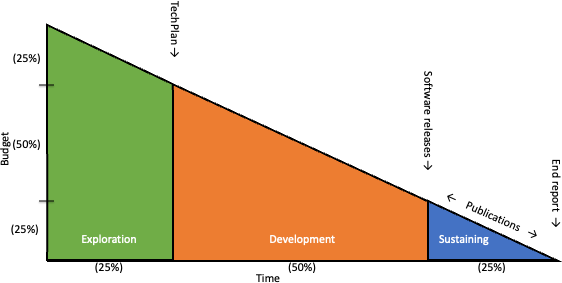
\includegraphics[width=0.97\textwidth]{img/budget-stages.png}
        \vspace{0.2cm}
        %\caption{Standard}
    \end{subfigure}%
    \hfill
    \begin{subfigure}[b]{0.49\textwidth}
        \centering
        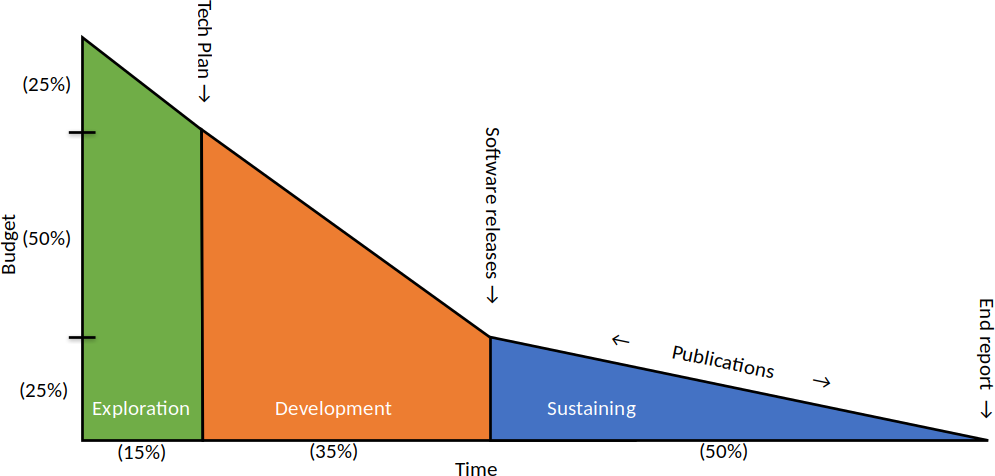
\includegraphics[width=0.97\textwidth]{img/budget-faster.png}
        \vspace{0.2cm}
        %\caption{Fast}
    \end{subfigure}
    \caption{Project's budget breakdown: standard (left) and fast (right)}
    \label{fig:project-budget}
\end{figure*}

The eScience project team (including PM and RSEs) must submit project hours in Exact by the end of each month. All entries must be completed within one working week after month-end. 
%Hours must be submitted and approved on time, preferably on a weekly basis.
%
For regular call projects, RSEs can write hours once the project is active in Exact, typically within a month of grant approval. The PM records management hours on the project budget. 
%
Project hours are managed by different parties with different responsibilities:%, see Table~\ref{tab:budget}.
\let\myhcolw\relax 
\newlength{\myhcolw}
 \setlength{\myhcolw}{0.6\textwidth}
\begin{table}[!htb]
% \caption{Parties at the eScience Center and their responsibilities}
\renewcommand{\arraystretch}{1.5}
\begin{booktabs}{colspec={|p{0.1\textwidth}|p\myhcolw|p{0.3\textwidth}|},row{even}={gray!20}}
    \toprule
    \textbf{Stakeholder} &  \textbf{Responsibilities} & \textbf{More info} \\\toprule
    PM & 
    \begin{minipage}[t]{\myhcolw}
    \begin{itemize}[itemsep=-4pt,parsep=4pt,leftmargin=0.5cm]
        \item reviews and approves project hours by the 5th workday of the following month.
        \item shares monthly hour status with RSEs via Ganttic
        \item flags issues (e.g., incorrect budgets) to Finance
        \item notifies Finance of budget changes.
    \end{itemize} 
      \end{minipage}
    & \\\midrule
    Lead RSE &     
    \begin{minipage}[t]{\myhcolw}
    \begin{itemize}[itemsep=-4pt,parsep=4pt,leftmargin=0.5cm]
        \item monitors project hour expenditure 
        \item signals deviation from the workplan to the PM
    \end{itemize} 
      \end{minipage}
    &  %Asks PM for hours status in Exact or via Ganttic  
    \\\midrule
    Finance &
    \begin{minipage}[t]{\myhcolw}
    \begin{itemize}[itemsep=-4pt,parsep=4pt,leftmargin=0.5cm]
        \item maintains accurate budget information 
        \item monitors and processes approved project hours
        \item shares monthly financial info with budget holders (PMs). 
        \item recalculates project budget if extended past year threshold.
        \item sets project to read-only if hours are depleted/exceeded early.
    \end{itemize} 
      \end{minipage}  
    & All budget changes require a formal decision (see~\ref{sec:exec:changes}). \\\midrule
    DoT & 
    \begin{minipage}[t]{\myhcolw}
    \begin{itemize}[itemsep=-4pt,parsep=4pt,leftmargin=0.5cm]
        \item monitors and approves software sustainability hours 
    \end{itemize} 
      \end{minipage}
    & There is a separate protocol on handling software sustainability. \\
    \bottomrule
\end{booktabs}
%\label{tab:budget}
\end{table}

It is possible to travel for a project, however RSEs must ask approval of their line managers (a respective SH) before
committing to an event requiring travel and fill out a travel form. See the Intranet for more information.

For \textbf{external projects}, only the PM and RSEs formally working on the project may write hours. Some projects 
(e.g., Horizon Europe) allow only direct project activities -- non-project activities like SIG involvement cannot be charged on the project. 
The Lead RSE and PM must know these restrictions or consult Finance if unsure.

\subsection{Workshops}
\label{sec:exec:workshops}

Some call projects require the LA to organize workshops. These workshops aim at fostering research communities around
the software developed in projects. Workshops may focus on early user feedback, new features, or connecting existing tools to broader communities. 
%
Based on the call text, the PM and Lead RSE determine whether one of more workshops must be organized. 
Finance provides the project's workshop budget status. There are two types of workshops, namely, (a) organised by the LA, and (b) organized by the Lorentz Center.
%
\paragraph{For workshops organized by the LA:} the LA writes and submits the workshop plan(s) to Finance in a timely manner 
(see~\cite{proj-portfolio} for templates). Finance approves the plans in consultation with the PD and PM. 
The Lead RSE is expected to contribute to the workshop and its organization. A CM can advise the LA (through the Lead RSE) on
fostering engagement and growth of relevant software communities; a CM is involved in the introductory
part of the workshop, including addressing attendees. Finance handles the administrative and financial aspects of the 
request and requests feedback on the scientific content from the PM team.


%Detailed procedure of workshops approval is described in Appendix~\ref{app:workshops}.
%
\paragraph{For workshops organised by the Lorentz Center:} the LA must apply through the Lorentz Center webpage.
%\footnote{The procedure is described in the eScience - Lorentz Center Agreement and Annexes {\textcolor{red}(add the link when signed)}.}.
%
The LA has the leading role in the application. The Lead RSE takes an advisory role in the writing and design of the
workshop proposal and is expected to actively participate during the workshop event. The PM must ensure enough hours
are allocated for the Lead RSE (or RSE from the project team) to help the LA with the proposal and attend the workshop,
if they want to take an active role.

These workshops differ from the eScience-Lorentz Center Competition workshops that are jointly funded by the eScience and
the Lorentz Center. Besides co-funding expenses, the eScience Center provides an additional in-kind support. 
The role of the eScience RSEs is described in the awarded proposals. The project
initiation and the eScience team assignment follow the usual process. The team
collaborates with the organizers on planning and outcome of the workshop (e.g. research paper, white paper, software
release, or grant consortia). The Lead RSE plays a pivotal role in preparing and
delivering the workshop, and, possibly, in publishing any outcome drafted during the event. 

\subsection{Data and Software Management Plans}
\label{sec:exec:mp}
For some projects, Data and Software Management Plans (DMP~\cite{dmp-guide} and SMP~\cite{smp-guide}) outline how project data and software are maintained. 
%
Depending on the call, the LA must submit complete DMP and SMP documents within 6 months of the project. The Lead RSE 
may assist in drafting the DMP, which the LA submits to the PM, who asks a TL for review and approval. For call projects since 2021, SMPs are included in project proposals.

The LA is responsible for keeping both plans up to date and must inform the PM and TL of changes via the Lead RSE. The PM may request updates as needed, with support from the Lead RSE.


\subsection{Knowledge transfer}

To increase visibility of the project and its results, the project team (including RSEs, PM, TL), Communications, CMs,
share knowledge and outcomes both inside and outside of the organization. The Lead RSE ensures that
\begin{itemize}
\item project results are timely shared with Communications, CMs, and relevant SH;
\item project and software pages on the RSD are properly updated; and
\item specific requests to facilitate project visibility are sent to Communications by RSEs.
\end{itemize}

Moreover, PMs, Lead RSEs and TLs work together to spot opportunities for cross project collaboration (e.g., by reusing
software or knowledge in these projects or as a new reusability project, read more in Section~\ref{sec:opportunities:ss}).



\subsubsection{Output management}
\label{sec:exec:output}
Project deliverables include research articles, presentations, talks, posters, tutorials, datasets, blog posts, white papers, and workshops, 
as well as software-related outputs such as code releases, software papers, demos, videos, tutorials, and training materials. 
%
RSEs strive to apply FAIR principles~\cite{fair-principles,FAIR4RS} to all project deliverables. They should have
\begin{itemize}\itemsep0em
\item (concept) DOIs from publishers or open-access archives like Zenodo, arXiv, or DANS;
\item acknowledge the eScience Center project grant~\footnote{By adding the following sentence into the publication: "<full project title> is a project of the Netherlands eScience Center, funded under grant number <grantid>."}; and
\item listed RSEs working on the project as (co-)authors.
\end{itemize}

RSEs must record all project outputs in relevant systems and databases (see Table~\ref{tblr:output}) to ensure knowledge transfer. 
The PM expects the team to follow the deliverables plan outlined in the proposal and workplan. RSEs contribute to publications and software/data releases.

\begin{longtblr}[
  theme = fancy,
  caption = {Output management},
  %entry = {Short Caption},
  label = {tblr:output},
%  note{a} = {It is the first footnote.},
%  note{$\dag$} = {It is the second long long long long long long footnote.},
  %remark{Note} = {Some general note. Some general note. Some general note.},
  %remark{Source} = {Made up by myself. Made up by myself. Made up by myself.}
]{
 % colspec = {|X|X|X|X|X|}, width = 1\linewidth,
  colspec={|p{0.12\textwidth}|p{0.12\textwidth}|p{0.35\textwidth}|p{0.1\textwidth}|p{0.2\textwidth}|}, width = 1\linewidth,
  rowhead = 1, %rowfoot = 1,
  row{1} = {font=\bfseries},
  column{1} = {font=\bfseries},
  row{odd} = {white}, row{even} = {white},
  row{1} = {gray!20}, %row{Z} = {nlesc-yellow},
  %cell{2}{1,4,5} = {r=2}{t},
  cell{2}{1,4,5} = {r=2}{t},
  cell{4}{1,4,5} = {r=2}{t},
  cell{6}{1,4,5} = {r=3}{t},
  %cell{9}{1,4} = {r=2}{t},
}
\toprule
What & Responsibility of & Responsible for  & URL & Additional info \\
\toprule
Zenodo (NLeSC community) & PM / CMs  & curating and approving new publications & \href{https://zenodo.org/communities/nlesc/}{Zenodo link} & 
    \begin{minipage}[t]{1\linewidth}
    \begin{itemize}\itemsep0em
        \item Publications on Zenodo are added to the community
    \end{itemize} 
    \end{minipage}  \\
%\midrule
\cmidrule{2-3}
    & RSEs & getting a (concept) DOI for a data or software release, or a document (e.g., non-peer-reviewed publications) 
&  & \\
\midrule
RSD, software and project pages & PM / Lead RSE & 
    \begin{minipage}[t]{1\linewidth}
    %\vspace{-1cm}
    \begin{itemize}\itemsep0em
      \item ensure the eScience team has maintainer access 
      \item decide on reuse of the project page if the project continues under new funding.
    \end{itemize} 
    \end{minipage}  & 
    See \href{https://research-software-directory.github.io/documentation/introduction.html}{RSD intro} and
\href{https://github.com/research-software-directory/documentation/blob/main/docs/adding-projects.md}{Adding RSD project} &
  %Each project has its RSD project page. The Lead RSE in agreement with the PM can use the same RSD project if a direct continuation of the project is granted from another funding source. In this case, the funding source and respective text should be added. \\
  Each project has an RSD page. When reusing a project page under new funding, Lead RSE updates it with the new funding source and details.\\
\cmidrule{2-3}
    & RSEs &  
    \begin{minipage}[t]{1\linewidth}
    \begin{itemize}\itemsep0em
      \item create project page, if needed 
      \item maintain pages with complete, up-to-date metadata
    \end{itemize} 
    \end{minipage} &  & \\
\midrule
     Project portfolio & PM & adding a direct link to the project portfolio in Ganttic & 
     cf.~\cite{proj-portfolio} for structure explanation. &  
    An internal archive with regular automatic backups. Direct link to the portfolio folder available in Ganttic   \\
\midrule
    & Lead RSE & ensuring that all docs are available & & \\
\midrule
    & RSE & 
   \begin{minipage}[t]{1\linewidth}
    \begin{itemize}\itemsep0em
        \item upload outputs (e.g., papers, reports, presentations)
        \item link the source material in the project log
    \end{itemize} 
    \end{minipage} & &  \\
\midrule
%\pagebreak
  The eScience Center blog  & RSEs &  
  \begin{minipage}[t]{1\linewidth}
    \begin{itemize}\itemsep0em
        \item Create a blog post about the project, its progress, or outcomes.
        \item add final blog URL to project RSD page
    \end{itemize} 
    \end{minipage} &
  Indexed at \href{https://blog.esciencecenter.nl/}{eScience Blog} & Instructions on blogging are posted on the Intranet~\cite{intranet}
 \\
\midrule
      & Editorial Team & 
    \begin{minipage}[t]{1\linewidth}
    \begin{itemize}\itemsep0em
        \item Review blog post entry of project team 
        \item Help at any stage with writing and publishing process
    \end{itemize} 
    \end{minipage} & &   \\ 
% Foot    & &  &Foot  & Foot    \\
\bottomrule
\end{longtblr}


Open access publications and open source software are mandatory for all call projects. The PM and Lead RSE inform the LA if needed. 
Open access fees are budgeted by Finance annually in the call budget (with the PD approval); if no budget is available, alternatives can be explored:

\begin{itemize}\itemsep0em
  \item publishing through the LA's institution (either open access funds are available or the LA organization is connected to publish open access in a lot of journals through the library without a fee)
  \item choosing the best option for open-access publishing (is it a diamond or gold open-access journal)
  \item publishing closed access and self-archiving either a preprint or publication after six months under Taverne agreement in Dutch copyright law (cf.~\cite{taverne,taverne:ou}).
\end{itemize}
The Lead RSE and PM consult Finance regarding payments for an open access publication.

For \textbf{external projects} the expected deliverables are also part of the formal project documents (proposal,
contract, etc. The Lead RSE is expected to keep the PM informed of the status of deliverables throughout the project.


\subsubsection{Outreach}
\label{sec:exec:outreach}
The Lead RSE promotes the project's visibility through project demonstrators, presentations, and
other means. All RSEs are expected to communicate externally about the project and its deliverables, as
outlined in Section~\ref{sec:exec:output}. Communications supports the project team by 
highlighting project through various channels, including but not limited to news items, social media
posts, videos and interviews about relevant the scientific impact of the research software developed 
or used. The Lead RSE (or occasionally the PM) provides Communications with relevant information. 


Blog posts are an optional but highly recommended output of the projects. Any team member, from LA to RSE, can author them. 
Topics may include simplified research summaries, tutorials on learned skills or technologies, or updates on workshops, publications, and other project outputs.

RSEs share project progress and results (e.g., technology plan, milestones, code releases) with colleagues, 
including SIG presentations. Each RSE prepares and updates a 3-slide deck or pitch \cite{proj-portfolio}. 
The Lead RSE ensures a demonstrator is available after the first major software release.


The LA and their team are encouraged to participate in relevant Digital Skills Workshops~\cite{digital-skills} from the eScience Center. Furthermore, if the LA and their team
require a project-specific training workshop, the Lead RSE involves
\begin{itemize}
\item workshop coordination with CMs, who can advise on organization and training material development; Finance handles any related payments if applicable;
\item the PM discusses RSE hours spent on training organization and consults Finance if needed.
\end{itemize}

For \textbf{external projects}, consortium agreements (e.g., Non-Disclosure Agreement or NDA) may define result communication. The Lead RSE and PM review these at project start to clarify communication boundaries.

\subsection{Code quality and sustainability checks}
Ensuring software quality and sustainability is integral to the code development process cycle at the eScience
Center. All RSEs are expected to follow our software development guide and best practices~\cite{guide-nlesc}. Code should be 
designed to be as generic and reusable as possible from the start.

\subsubsection{Code development}
\label{sec:exec:code}
At the initial stage of code development in the project, the Lead RSE together with RSEs:

\begin{itemize}\itemsep0em
\item set up a GitHub organization for the project, following the eScience Center Guide and the Turing Way~\cite{the_turing_way-2023}
\item add the URL of this organization to the RSD project page.
\end{itemize}

RSEs must always ask at least one project team member, relevant SIG member or other RSE at the eScience Center to
review, comment and approve pull requests in the project codebase.

\subsubsection{Code review}
As part of the annual review (see Section~\ref{sec:exec:annual}), a code review is organized by the Lead RSE. Depending
on the project it could take the form of a reusabilithon\footnote{Coined by the Software Sustainability SIG, the term refers to a 2-3 hour session where a group of RSEs evaluates a piece of software for usability, provides feedback to the developers, and formulates recommendations to improve its (re)usability.}, a review of code on GitHub, or
something else entirely (format to be approved by TL). The reviewers for this process are typically other RSEs at the
eScience Center.


The goal is to review software of the project for:
\begin{itemize}\itemsep0em
\item its usability (reproducing steps of installations, and running it on a machine/laptop)
\item overall software quality and suitability
\item whenever appropriate, correctness of code
\item adherence to the technology plan (Section~\ref{sec:init:techplan})
\item adherence to eScience Center best practices
\item opportunities for reuse of software in other projects
\item correct inclusion in output systems (Section~\ref{sec:exec:output}).
\end{itemize}

Reviewers make written suggestions for improvements, and flag major issues encountered. These issues serve as input for
the TL for the formal annual review meeting (see Section~\ref{sec:exec:annual}). These notes are stored in the project log. 

\subsection{Annual project review meeting}
\label{sec:exec:annual}

\let\myhcolw\relax % let \myhcolw to \relax to be reused later
\newlength{\myhcolw}
\setlength{\myhcolw}{0.75\textwidth}

\begin{table}[h!]
\begin{booktabs}{colspec={|>{\bfseries}m{0.2\textwidth}|m{\myhcolw}|},row{even}={gray!20}}
    \toprule
    Scheduled: &  Yearly \\[1.5ex]
    Stakeholders: & PM (organizer, chair), Lead RSE, LA, TL, optional: other project team members, SH \\[1.5ex]
    Purpose: &  %
    \begin{minipage}[t]{\myhcolw}
    \begin{itemize}[leftmargin=0.3cm]\itemsep0em
        \item to ensure that the project is still on track
        \item to discuss any persistent issues to ensure optimal collaboration between project team
        \item to explore opportunities beyond the project  
    \end{itemize} 
      \end{minipage}
    \\[1.5ex]
    Outcomes/Actions: & List of agreed actions and PM/TL advice for next steps. \\[1.5ex]
    Duration: &  Max 1.5 hours \\[1.5ex]
    Location: &  At the eScience Center or the project location\ftnotelbl{ft:participants} \\[1.5ex]
    \bottomrule
\end{booktabs}
\end{table}
%\footnotetext[2]{Mandatory participants of a meeting be present in-person at the office, while all optional participants can also participate via video conferencing if they prefer.}


For call projects longer than one year, the PM organizes annual reviews. The details are described in the
terms and conditions document~\cite{nlesc-terms}. For one-year projects, review meetings are optional and decided by the PM in consultation with the TL and Lead RSE.

Each review includes discussion and actions on reusability and sustainability of project results (as described in the DMP and SMP), status of collaboration, and follow-up opportunities. 
%
\iffalse
The goals of the meeting are to:
\begin{itemize}
\item review progress against the original workplan
\item discuss research results, their novelty and current deliverables
\item update management plans if needed
\item plan strategies to share results with a wider community
\item address software reuse and sustainability
\item identify bottlenecks and improvements for team efficiency
\item report project financials (RSE hours remaining)
\item explore further collaboration, funding, and cross-project opportunities
\end{itemize}
\fi
The agenda of this meeting is:
\begin{itemize}\itemsep0em
\item introduction and purpose of meeting
%\item project overview and deliverables
%\begin{itemize}
\item scientific goals status (the LA and team)
\item project output status (the project team)
%\end{itemize}
\item collaboration status (including hours admin and bottlenecks)
\item use of digital infrastructure and SURF support (if applicable)
\item next steps and future opportunities.
\end{itemize}
For \textbf{external projects}, review meetings are typically part of the project process. The PM, with the Lead RSE, decides if a (lightweight) internal review is needed.


\subsubsection{Review meeting preparation}
\begin{table}[h!]
  \renewcommand{\arraystretch}{1.5}
\begin{booktabs}{colspec={|>{\bfseries}m{0.3\textwidth}|m{0.6\textwidth}|},row{even}={gray!20}}
    \toprule
     &  \textbf{Stakeholder} \\[1.5ex]\toprule
    Prepared by: & LA and Lead RSE, with optional input from other stakeholders. \\[1.5ex]
    Reviewed by: &  PM accountable for project, TL accountable for technology. \\[1.5ex]
    Target audience: & PMs, TLs, SHs and RSEs. \\[1.5ex]
    \bottomrule
\end{booktabs}
\end{table}

The Lead RSE coordinates preparations for the review meeting:
\begin{itemize}\itemsep0em
\item request the PM to share the standard review meeting slide template~\cite{proj-portfolio} with the LA team
\item requests project team members to contribute to the review meeting slides, wherever appropriate,
\item compiles technology status report (see Section~\ref{sec:exec:tech}).
\end{itemize}


LA and Lead RSE jointly prepare the slides:
\begin{itemize}\itemsep0em
\item 3-5 slides summarizing progress toward research goals. The LA is not expected to present published content or the
original workplan or proposal. If applicable, the LA reports on workshops.
\item 1-2 slides on the technology plan status, including reuse, adoption, and sustainability, supporting the technology status report.
\item highlight any scientific or technical bottlenecks and assess if the project is on track or needs replanning;
\item the PM reports on the RSE hour status (i.e. the number of hours already spent); and
\item the project team provides a feedback on collaboration and suggest improvements if needed.
\end{itemize}
 
Additionally, the Lead RSE:
\begin{itemize}\itemsep0em
\item together with the LA, ensures all output is properly registered (see Section~\ref{sec:exec:output}), and adds missing URLs/DOIs to the slides;
\item coordinates with the team to finalize the presentation at least 2 working days before the review meeting;
\item uploads the slides to the project portfolio; and
\item informs PM and TL that slides are ready and are in the project portfolio.
\end{itemize}

\subsubsection{Technology status report}
\label{sec:exec:tech}
Prior to the annual review meeting, the PM asks Lead RSE to fill in the technology status report. This report 
summarizes the technical progress of the project and includes RSD project page with its deliverables, URLs
to project plans, software quality and community involvement. The Lead RSE prepares it in collaboration with the project team; it serves as input for the TL during the review.

The Lead RSE:
\begin{itemize}\itemsep0em
\item collects output and relevant information from LA and team
\item meets with CM to draft the technology status report  
\item draft the rest of the report with the TL
\end{itemize}

Two weeks prior to the review meeting, the Lead RSE submits the completed report to the TL. The TL conducts a code 
review or software health check based on the report and shares the results with the eScience team. If needed, 
the Lead RSE, TL, and PM may meet to discuss the findings before the annual review meeting.

The report and the review(s) are archived by the TL in the project portfolio.

\subsubsection{At the review meeting}
The time breakdown of the meeting agenda is follows:
\begin{itemize}\itemsep0em
\item presentation by the LA (max. 20 min)
\item presentation by the Lead RSE (max. 20 min), including the RSE roles and deliverables
\item discussion (max. 40 min)
\item summary, action points and conclusions.
\end{itemize}

The PM chairs the meeting and, with the TL, acts as reviewer. The TL highlights tech/software issues. Everyone contributes to the discussion. PM and TL assess deliverables, and comment on their status:
\begin{itemize}\itemsep0em
\item have the objectives outlined in the proposal been sufficiently addressed? (PM)
\item does the project follow the workplan in terms of deliverables? (PM)
\item has the output been registered according to the rules of output management (Section~\ref{sec:exec:output})? (PM, TL)
\item does all project output have publications (including software and data papers)? (PM)
\item are there any issues flagged during the code review that needs to be discussed with the project team? (TL)
\item does the project team sufficiently engage and align with relevant communities (e.g., via the workshops)? (PM)
\item does the project adhere to the technology plan, SMP and DMP? (TL)
\end{itemize}

The eScience project team comments on any further possibilities for reusability, adoptability and sustainability of the
software, and the project team comments on possible collaborations beyond the project.

The PM updates the slides with action points, agreements and plans (with the project partners agreement). The PM logs
the meeting in the project log.

\subsubsection{After the review meeting}
PM shares the updated slide deck with the project team members to check the agreements written down. PM ensures that the
final version of the presentation(s) uploaded to the project portfolio is correct.

\subsection{Reporting}
\label{sec:exec:report}
For call projects the annual review meeting and end report (Section~\ref{sec:closing}) serve as formal progress reports.

\textbf{External projects} may require periodic reporting to the consortium on progress and deliverables. 
The PM and Lead RSE consult the agreements, contract, and workplan; Finance handles financial input. 
The external coordinator (e.g., EU project coordinator, NWO programme officer) signals deadlines on the report delivery. 
The Lead RSE drafts the eScience Center's contribution, the PM reviews it. Finance fills in the financial part of the report 
(signed by the DoO if needed). The PM submits the final report to the external project coordinator 
(via EU portal done by Finance) and archives it in the project portfolio.

\subsection{Conflict resolution and complaint procedure}
The eScience Center adheres to the Code of Conduct outlined in the Personnel Policy (cf.~\cite{cao}). 
%
Conflicts involving eScience and the LA team on the projects should be addressed using this four-step process:
\begin{enumerate}\itemsep0em
\item The Lead RSE first seeks resolution with the LA; the PM may be consulted or join in discussion if needed.
\item If unresolved, the issue is escalated to the PM (via the Lead RSE), who organizes a meeting to mediate.
\item Persistent issues can be escalated to the PD via a written summary submitted through the PM.
\item The PD may escalate to the DT if necessary.
\end{enumerate}

If the issue concerns the PM, RSEs may escalate to their manager (SH). An external confidential advisor ('Vertrouwenspersoon') is also available for anonymous support~\cite{intranet}. 
Conflict resolution may lead to project adjustments, such as staffing changes (cf. Section~\ref{sec:init:vacancy}).

\subsection{Non-RSE Consultants}
\label{sec:exec:consult}
Certain issues require consultation beyond the project team. Team members must inform the PM, who may delegate actions as needed:

\begin{itemize}\itemsep0em
\item GDPR/personal data: consult the GDPR contact~\cite{intranet}. 
\item Software/data quality and access: contact the TL.
\item Scientific integrity: contact the integrity officer~\cite{intranet}.
\item SURF-related matters: contact SURF liaisons~\cite{intranet}.
\item Sustainability: contact TL and CMs.
\item IP/licensing: contact TLs and DoT. (cf. Section~\ref{sec:init:kickoff}).
\item Legal matters: contact the DoO (cf. Section~\ref{sec:init:legal}).
\item External funding/opportunities: contact the PD (cf. Section \ref{sec:opportunities:external-funding}).
\end{itemize}

\subsection{Changes to the project}
\label{sec:exec:changes}
During the project life cycle, the workplan may change substantially:

\begin{itemize}\itemsep0em
\item New deliverables because of additional funding
\item New workplan because of changes in the research goal and/or in the technology used
\item Timeline, leading to a different end date.
\end{itemize}

Any of these changes needs explicit approval from the PM team or the DT.


\begin{table}[h!]
\begin{booktabs}{colspec={|m{0.65\textwidth}|m{0.3\textwidth}|},row{even}={gray!20}}
    \toprule
     \textbf{Type of request} &  \textbf{Decided by:} \\[1.5ex]
    Budget requests within the PM mandate~\cite{intranet} & PM team \\[1.5ex]
    All requests regarding budget changes outside the PM mandate &  DT (via PD) \\[1.5ex]
    Early termination & DT (and DT informs the Board) \\[1.5ex]
    \bottomrule
\end{booktabs}
\end{table}


For \textbf{external projects}, changes must follow the formal agreements (e.g., grant or consortium agreement). 
The PM handles extensions within their mandate or escalates to the DT. The PM informs the external funder or consortium of the outcome.

\subsubsection{Proposal changes request}
The LA must submit a formal request to the PM team (by email via the PM, in PDF format, signed) containing:

\begin{itemize}\itemsep0em
\item project title and project number
\item requested change (e.g., time/dates, RSE hours, scientific goal) and motivation for this change
\item conditions such as deliverables: any new deliverables should have updated timeline. If none, state explicitly.
\item any motivated budget change, such as 
\begin{itemize}
\item LA wants to increase their involvement 
\item change in research personnel (if applicable in the case of older projects)
\item transfer between hardware and PYR for RSE or LA personnel costs (if applicable, for older projects)
\item any in-kind to cash change, or vice versa (including requests with the extra cash budget from the LA).
\end{itemize}
\item any prior or planned inactivity on the project, such as
\begin{itemize}
\item personnel shortage on the LA side due to maternity/sick leave or hiring delays (but there is a concise timeline on the hiring procedure)
\item unavailability of RSEs 
\item additional data that needs to be collected.
\end{itemize}
\item any delay with the start date.
\end{itemize}


\subsubsection{Processing the changes request and decision}
Upon receipt of the request, the PM assesses if the request should be granted based on considerations such as 
\begin{itemize}\itemsep0em
\item whether the new objective is scientifically promising or technologically interesting? (if applicable)
\item collaboration status with the LA;
\item prior problems regarding the project;
\item benefits for the eScience Center (e.g., smooth wrap-up, future funding opportunity); and/or
\item availability of RSEs with relevant expertise to work on it.
\end{itemize}

The PM can consult with RSEs and the TL on whether the new planning is feasible, and with Finance for a budget remaining after necessary recalculation. In case of additional funding, the DT
(via the PD) will decide, after a budget calculation by the Finance and approval by the DoO. Otherwise, the PM puts the
request on the agenda for the next PM meeting, containing: 
\begin{itemize}\itemsep0em
\item the motivated request (uploaded to the project portfolio
\item the recommended action
\item the prepared decision on the PM meeting agenda.
\end{itemize}

The PM team may request more information from the LA via the PM (and thus postpone the decision on the request). The LA
can provide the new information via an additional PDF signed letter or as amendment to the original letter.

After the final decision, the PM notes the official decision in the decision document. If the request is not approved,
the PM communicates this to the LA. If the request is approved, the PM
\begin{itemize}\itemsep0em
\item coordinates with Finance to finalize the extension (budget/Exact update, extension letter, LA communication);
%\item double checks if budget and hours in Exact are still correct;
\item communicates the extension to the Lead RSE.
\end{itemize}  
  The Lead RSE then 
\begin{itemize}  
\item communicates the extension to the project team;
\item updates planning and adjusts staffing, if necessary;
\item ensures website and RSD are updated (e.g., if dates or affiliation changed); and
\end{itemize}

If the request involves a DT decision, the PM submits a request formally through the PD.

\subsubsection{Early project termination}
Early project termination may occur by mutual agreement, or be initiated by the LA or the eScience Center. In the first two cases, 
the LA submits a signed letter (via the PM) to the DT, requesting project termination, explaining the situation and proposing how to 
handle remaining project resources (e.g., RSE hours, cash contribution, FTE commitment of the LA, workshops, sustainability budget).

The PM may request project termination if the LA or project partners violate the terms of Awarding Letter or Special conditions ("Bijzondere Voorwaarden"). 
The PM submits a letter with the explanation to the DT via the PD. If approved, the PM informs Finance, which finalizes the process (by making changes in Exact and preparing a termination letter).

\subsection{Opportunities beyond the project}
\label{sec:opportunities}
A project team can explore different opportunities for ideas that stem from the project that go beyond its scope and/or
budget. Appendix \ref{app:pm-role} summarizes the role of PM in such projects. The PM discusses these opportunities with the project
team during the review meeting.


\subsubsection{Increasing reusability (in this document called software sustainability)}
\label{sec:opportunities:ss}
Some projects or calls have dedicated software sustainability budgets~\cite{nlesc2024software}. Until 2020, each project 
received its own Generalization (“Generalisatie”) budget for reuse of project results.
Since 2020, this budget is allocated at the programme or call level. The PM and Lead RSE must check the call text, awarding 
letter to confirm its availability.

The PM signals potential for reuse to the TL, who discusses it with the Lead RSE and, if needed, the TL team. 
RSEs with ideas for sustainability projects can contact the TL or DoT. The process follows the SS protocol~\cite{intranet}.

\subsubsection{Knowledge and Development}
\label{sec:opportunities:kd}
For the development of broad and deep knowledge on digital technologies and their application, RSEs can apply for
so-called Knowledge and Development (KD) project. The process is described by the KD protocol~\cite{intranet}.

\subsubsection{External funding}
\label{sec:opportunities:external-funding}
The project team may decide to pursue other funding opportunities. The eScience Center encourages RSEs to pursue
external funding opportunities to promote the organization profile as research organization. PD oversees the
Acquisition activities and the process. The relevant information is available via Intranet~\cite{intranet}.


\subsubsection{Fellowship}
\label{sec:opportunities:fellowship}
To stimulate community engagement lasting longer than project lifetime, the eScience Center funds annual Fellowship
Program~\cite{fellowship,fellowship-call}. The eScience project team is not eligible for this program, however, the LA and their team are.

\clearpage

\section{Project closing}
\label{sec:closing}
Project closing is the final phase of a project. In this phase the PM (with the help of F\&C) processes the end report
and accepts the project deliverables. Once the project is formally closed, RSEs can no longer write hours or work on
this project. 



\subsection{End report}
\label{sec:closing:end}
All completed call projects at the eScience Center must have an end project report.

\begin{table}[!h]
\begin{booktabs}{colspec={|>{\bfseries}m{0.2\textwidth}|m{0.8\textwidth}|},row{even}={gray!20}}
    \toprule
    Written by: &  the LA, assisted by the Lead RSE. \\[1.5ex]
    Target audience: & PMs, RSEs, Communications (layman summary), F\&C (accountants), TLs \\[1.5ex]
    Schedule: &  %
    \begin{minipage}[t]{0.8\textwidth}
    \begin{itemize}\itemsep0em
        \item written in last months of the project,
        \item submitted 3 months after the project end at latest, 
        \item archived in the project portfolio on the internal All SharePoint site. 
    \end{itemize} 
      \end{minipage}
    \\[1.5ex]
    Approved by: & The PM team and F\&C. \\[1.5ex]
    \bottomrule
\end{booktabs}
\end{table}

The Lead RSE and RSEs can assist the LA in writing the end report, providing necessary information for it (such as
deliverables). A complete end report (in PDF format, using a template provided by the PM) contains:
\begin{itemize}
\item lay summary (written in English)
\item scientific summary with clearly stated objectives/results
\item a list of deliverables and project outcomes (e.g., software, papers, presentations, pitch), including list of workshops
(if applicable) 
\item remarks on sustainability of project results and the latest version of the management plans
\item financial report (if applicable)
\item signature of the LA and date of signing (in case the PM cannot get the LA signature, a signature of financial or project
manager would also be acceptable).
\end{itemize}

For collaborative call projects, the end report written by the LA and the Lead RSE for the other funder (e.g., NWO) is
sufficient, if it contains all necessary information, covered by the bullet list above.

For \textbf{external projects} the way a project is formally closed depends on the formal documentation for a project.
Often a final report is required for the external funder. The Lead RSE contributes to this report (PMs can assist when
needed), and care should be taken to reserve some time (and budget) during the project for this effort. F\&C assists
with the financial part of the reporting. The necessity of a (lightweight version of an) internal end report is
determined by the PM and F\&C.

The Lead RSE ensures all output is registered in the appropriate systems (see Section \ref{sec:exec:output}) before the
PM team will accept the end report.

Projects that are funded by software sustainability budgets have their own procedure for end reports (see Appendix
\ref{app:pm-role}.). The end report of these projects consists of output registered on the RSD project page and
updated summary of the project.



\subsubsection{Requesting end report}
For call projects, one month before the project end, the PM requests the LA to submit the scientific and financial end
report ('Financieel en wetenschappelijk eindverslag'), providing the
template~\cite{proj-templates}. The LA submits the report to the PM \textit{no later than three months after} the project end date.


For an \textbf{external project}, the PM requests the Lead RSE to write the report or share the end report written for
the external party or funder (e.g., EU, NWO). In this case, F\&C prepares the financial part of the report. F\&C
periodically sends a list of missing end reports to the PM team. If the end report is not submitted yet, the PM sends a
reminder to the LA.

\subsubsection{Checking end report}
The PM reviews the report and fills in the review document (both templates are in the templates folder in the project
portfolio).

The checklist includes but is not limited to
\begin{itemize}
\item all items from Section~\ref{sec:closing:end} are present and satisfactory;
\item all output (e.g., papers, software, code) is stored properly and according to the rules in output management (Section
\ref{sec:exec:output});
\item all URLs are working;
\item papers are uploaded by the Lead RSE to the project portfolio in the Products subfolder; and
\item all entries in output systems (from Section \ref{sec:exec:output}) are complete.
\end{itemize}

F\&C reviews the financial report and either approves it or requests corrections to the report. If the end report is not
satisfactory, the PM asks the LA and/or Lead RSE for additional information or corrections to the report, before
resubmitting it to F\&C. 

PM and F\&C archive the end report and review form in the respective project portfolio folder (see Appendix
\ref{app:folders}.).

\subsection{Formally closing the project}
The PM puts decision to formally close project on the PM meeting agenda. After the formal decision\footnote{Formally
recorded by the PM team, and thereafter ratified by the DT team (see more in Appendix \ref{app:pm-mandate}.).}, the PM
notifies the TLs, F\&C and Communications (with the links to the documents). F\&C handles the approved reports and
formalities related to closing the project. This includes getting the final signature by DoO or Executive Director on
the official letter for the LA about the project closing ('Afsluitingsbrief').


The PM ensures that the project is marked as complete on the 
\begin{itemize}
\item RSD: The Lead RSE updates the project page with the summaries (from the end report) and sets the project status to
'Closed'. 
\item Corporate page: Communications may also request more information to promote the completion of the project through
various channels, including but not limited to a news item, social media post, video and interview.
\item Exact/Project portfolio: F\&C closes the Exact project budget, uploads the official closing letter to the LA, as well as
all appropriated documents, and moves the project folder in Project Portfolio to the Closed project folder.
\item Ganttic: The PM ensures that no one is assigned to the project in the future.
\end{itemize}


%bibliography section rename
\renewcommand{\bibname}{Related links and references}
\renewcommand{\bibsection}{\section*{\bibname}}

\bibliographystyle{abbrv}
\bibliography{references}


\clearpage

\appendix
{\color{nlesc-blue}\appendixpage}
\addappheadtotoc

\section{Lead RSE role description}
\label{app:leadRSE}

\textit{This role description includes guidelines that need to be followed by RSEs fulfilling the role; they will be
complemented by protocols.}

\let\myhcolw\relax 
\newlength{\myhcolw}
\setlength{\myhcolw}{0.7\textwidth}

\begin{table}[h!]
\begin{booktabs}{colspec={|m{0.25\textwidth}|m{\myhcolw}|},row{even}={gray!20}}
    \toprule
     1. Role &  Lead RSE \\[1.5ex]
     2. Place in the organization & Project \\[1.5ex]
     3. Contacts &  PMs, project team RSEs, external project partners, TLs, \\[1.5ex]
     4. Purpose & To carry responsibility for the day-to-day running of a research project at the eScience
Center and act as main contact point for the project. Each project has one Lead RSE.\\[1.5ex]
     5. Main tasks \& responsibilities & %
    \begin{minipage}[t]{\myhcolw}
    \begin{itemize}\itemsep0em
        \item Coordinating day-to-day activities with other RSEs working on the project;
        \item Carrying responsibility for agreements with the accountable PM on the division of tasks and
the allocation of time within the project;
        \item Making sure that activities, procedures and targets agreed upon are carried out and met on time;
        \item Monitoring project progress, including project hour expenditure, and regularly reporting progress to the accountable PM;  
        \item Ensuring the presence of the accountable PM at all formal meetings;
        \item Ensuring that general technological solutions are approved by the PM after due consultation
of TL, and monitoring their implementation;
        \item Ensuring that generalization and re-usability opportunities are implemented from the start of the project, after due consultation of TL and on approval
of the accountable PM;
        \item Solving everyday technical and managerial problems, and, if needed, communicating these to the PM;
        \item Ensuring the visibility of the project through project demonstrators, slide decks and other means; and/or
        \item Making sure all project output is properly released, documented and archived in the designated systems.          
    \end{itemize} 
      \end{minipage}
    \\[1.5ex]
    6. Competencies &  %
    \begin{minipage}[t]{\myhcolw}
    \begin{itemize}\itemsep0em
        \item Negotiating
        \item Communicating
        \item Cooperating
        \item Leading 
        \item Result orientation
        \item Planning and organizing
    \end{itemize} 
      \end{minipage}
    \\[1.5ex]
    7. Available resources (budget, hours, training) & In project budget\\[1.5ex]
    8. How to get this role & PM assigns Lead RSE based on skills, experience, knowledge, interest and availability, after prior consultation of SH.\\[1.5ex]  
    \bottomrule
\end{booktabs}
\end{table}

\let\myhcolw\relax % let \hcolw to \relax

\clearpage

\section{PM mandate to make changes in projects}
\label{app:pm-mandate}


On 04-07-2023, the DT team has approved the following 
\subsection*{PM Mandaat voor veranderingen aan projecten}
Het DT mandateert het Programme Management (PM) Team besluiten betreffende
aanpassingen van lopende projecten te nemen zonder tussenkomst van het DT, indien de aanpassingen zijn van de volgende
aard:
\begin{itemize}
\item Budget-neutrale vertragingen van de start van het project;
\item Budget-neutrale looptijdverlengingen;
\item Budget-neutrale verschuivingen (cash-cash, cash-kind, of kind-kind) tussen kostenposten binnen het project met een maximale
geldswaarde van 20\% van het gehele projectbudget en het totaal van 50.000 EUR niet overstijgend.
\item Veranderingen van Lead Applicant waarbij de nieuwe Lead Applicant al lid is
van het huidige consortium/project team
\item Veranderingen van organisatie van de Lead Applicant indien deze verandert van organisatie
\end{itemize}

Het PM team neemt deze besluiten in consensus. Indien deze consensus niet
bereikt wordt, beslist de programmadirecteur. Besluiten over projectaanpassingen die niet onder dit mandaat vallen,
worden genomen door het DT.

Alle besluiten betreffende aanpassingen van lopende projecten zoals hierboven
bedoeld dienen door het PM Team te worden medegedeeld aan de afdeling Operations (Finance).

Als onderdeel van het bovenstaande mandaat dienen tenminste elke 6 weken de
door het PM Team genomen besluiten aan het DT te worden voorgelegd ter informatie.


\clearpage

\section{Role of PM and others in external and Ambition 2 projects}
\label{app:pm-role}

This section focuses specifically on the role and involvement of the PM team in Fellowship,
External, KD, SS and D\&C projects.


\subsection{Fellowship projects}
Funded through the calls budget, Fellowship projects differ in purpose and organization from regular 
call projects. CMs are responsible for these projects, and a PM assigned by the PM team is advising them.

\subsection{External projects}

\begin{enumerate}[label=\arabic*.,ref=\arabic*]
\item Acquisition
\begin{itemize}
\item The eScience Center staff must follow the external funding policy and seek permission before pursuing an acquisition opportunity, in consultation with a PM.
\item During this consultation, the PM  must be informed of:
\begin{itemize}
\item estimated workload in person-hours
\item team composition and whether the person submitting the proposal  intends to serve as Lead RSE
\item timeline of the proposal/project
\end{itemize}
\item The PM can advise the Lead RSE on the proposal. If the advice is critical, the PM informs the PD. 
If additional (temporary) capacity is needed, the PM contacts the relevant SH. 
Note: planning remains provisional at this stage.
\end{itemize}
\item Preparation of project – call/subsidy projects
\begin{itemize}
\item The Lead RSE informs the PD, Finance, PM, SH, and relevant parties immediately upon granting confirmation.
\item The PD, Finance, and Lead RSE handle grant, consortium agreements, and project start documents.
\item The PM agrees on planning with the Lead RSE and the project team, and puts it in Ganttic.
\end{itemize}
\item Preparation of project – contract projects
\begin{itemize}
\item The Lead RSE and Finance arrange the contract, the Lead RSE keeps the PM informed of start dates.
\item The PM agrees on planning with the Lead RSE and the project team, and records it in Ganttic
\end{itemize}
\item During the project
\begin{itemize}
\item See the protocol for the relevant parts. The PM acts in consulting role and Lead RSE is
accountable.
\end{itemize}
\item Reporting
\begin{itemize}
\item As noted in Section~\ref{sec:exec:report}, the PM reviews the report. The Lead RSE or the grant applicant is responsible for obtaining the financial report from Finance and sending it to the external coordinator.
\end{itemize}
\item Closing of project
\begin{itemize}
\item Lead RSE informs PM of closing of project for funder or end of contract
\item PM follows formal closing steps as described by Section \ref{sec:closing}.
\end{itemize}
\end{enumerate}




\subsection{KD and SS projects}
The process for KD and SS projects is fully described by the KD and SS protocols~\cite{intranet}, respectively.
\begin{enumerate}[label=\arabic*.,ref=\arabic*]
\item Call and selection
\begin{itemize}
\item Follows the protocol
\item Upon granting, DoT or TLs inform Finance (cc PMs) which projects to create in Exact.
\end{itemize}
\item Preparation of the project
\begin{itemize}
\item The PM formally assigns the Lead RSE, discusses planning with the team, and enters it in Ganttic.
\end{itemize}
\item During the project
\begin{itemize}
\item The PM is not directly involved in the project unless requested by Lead RSE.
\end{itemize}
\item Reporting
\begin{itemize}
\item The extent of reporting is decided upon by DoT and TLs.
\end{itemize}
\item Closing of project
\begin{itemize}
\item Lead RSE informs PM of closing of project
\item PM follows formal closing steps, as described in Section \ref{sec:closing}.
\end{itemize}
\end{enumerate}

\subsection{D\&C projects}
D\&C projects for external funding follow the same process as other external projects.

The process for the D\&C projects for training and workshops is as follows:
\begin{enumerate}[label=\arabic*),ref=\arabic*]
\item Each October, the D\&C training lead provides SHs and PMs with an overview of training hours, including estimates for externally funded training.
\item SHs coordinate with RSEs on next year's training plans, ensuring total hours match D\&C projects needs. SHs share the planning 
with PMs and the training lead, and PMs incorporate it into projects planning.
\begin{enumerate}[label=\alph*.,ref=\alph*]
\item If training activities put project progress at risk, the PM alerts the SH. Together, they decide whether to reassign the training or the project to another RSE.
\end{enumerate}
\item During the year
\begin{enumerate}[label=\alph*.,ref=\alph*]
\item If an RSE exceeds their agreed upon training hours, the SH is responsible for discussing this
issue with the RSE and taking appropriate measures.
\item If a project is (unexpectedly) progressing unsatisfactory due to the RSE involved in training,
the PM discusses this with the SH and the RSE and takes appropriate measures.
\item If requests for externally funded training exceed the annual estimate, the training lead consults PMs on scheduling before deciding to give the training.
\end{enumerate}
\end{enumerate}




\clearpage

\section{Project Portfolio and its Structure}
\label{app:folders}

The project portfolio of active projects is located in All SharePoint~\cite{proj-portfolio}. 
The structure looks as follows: for example, for the ShiCo project, the location on All SharePoint is

\bigskip
Documents {\textgreater} Projectportfolio {\textgreater} Projects {\textgreater} 27014909 Mining shifting concepts through time (ShiCo)

\bigskip
and with the subfolders structure:
\begin{itemize}[leftmargin=*,label={}]
   \item A - Start documents
   \item B - Planning
   \item C - Reviews
   \item D - Products
   \item E - End documents
   \item F - Coordinators
 \end{itemize}
Administrative information.docx

 \bigskip
where \textit{27014909} is Exact-code of the project, and \textit{Mining shifting concepts through time (ShiCo)} is the
project title. These subfolders contain different type of project-related documents:
\begin{table}[h!]
\begin{booktabs}{colspec={|m{0.4\textwidth}|m{0.5\textwidth}|},row{even}={}}
    \toprule
      \textbf{Subfolder} &  \textbf{Its purpose/content}\\[1.5ex]\toprule
      A - Start documents & Initial project documents such as project proposal, start form, Awarding letter, collaborative
agreement, contract, changes to the Awarding letter. \\[1.5ex]\midrule
      B - Planning &  Planning related documents such as administrative start slides, kick-off slides. \\[1.5ex]\midrule
      C - Reviews & Documents such as annual review slides, annual review meeting notes, reports for external
projects, code review meeting notes. \\[1.5ex]\midrule
      D - Products & Project output like Publications, presentations, etc.\\[1.5ex]\midrule
      E –End documents & Project closing related documents such as end report, closing letter, end report review
report.\\[1.5ex]\midrule
      F - Coordinators & Project log, official extension letters. \\[1.5ex]\midrule
      Root folder/ Administrative information.docx & Administrative information regarding the project. \\[1.5ex]
    \bottomrule
\end{booktabs}
\end{table}


\clearpage

\section{Example of the project log}
\label{app:example-log}
\subsection*{Running log for Project XXX}

\begin{itemize}[leftmargin=*,label={}]
   \item 2022-03-12 Output: submitted paper
   \item 2022-02-02 Mr. X assigned as Lead RSE
   \item 2021-01-01 Kick-off meeting
   \item Present – NLesC: AB (PM), AA (Lead RSE), AC (TL), AD (RSE)
   \item Present – Team: FA (LA, TU Delft), PA (PhD student, TU Delft), RA (TU Delft)
   \item Agreements:
    \begin{itemize}
    \item Lorem ipsum dolor sit amet, consectetur adipiscing elit,
    \item sed do eiusmod tempor incididunt ut labore et dolore magna aliqua.
    \item Ut enim ad minim veniam, quis nostrud exercitation ullamco laboris.
    \end{itemize}
   \item 2021-02-10 SURF proposal granted 
   \item We received a grant (link) to infrastructure. We did not get Snellius access but were sent to Lisa as that also has
enough harddrives.
   \item 2021-02-02 SURF infrastructure proposal
   \item We submitted a proposal to SURF (talked to Henk). We decided to use Snellius as the harddrive in my laptop is too
small.
\end{itemize}

\bigskip


\subsection*{Project Start}

\begin{table}[h!]
\begin{booktabs}{colspec={|m{0.25\textwidth}|m{0.1\textwidth}|m{0.3\textwidth}|m{0.2\textwidth}|},row{even}={}}
    \toprule
      & \textbf{Date} &  \textbf{Slides/Meeting notes/URLs?} & \textbf{Notes} \\[1.5ex]\toprule
      Administrative Start meeting & 2021-01-01 & & \\[1.5ex]\midrule
      Project Kick-off & 2021-01-01 & & \\[1.5ex]\midrule
      Review1 & 2022-06-01 & & To plan final date\\[1.5ex]\midrule
      Review2 &  &  & \\[1.5ex]\midrule
      Tech plan v1 & 2022-06-20 & github.com/shico/techplan.rst & TL comments...\\[1.5ex]\midrule
      Paper & & & TODO: Add to RSD \\[1.5ex]\midrule
      Presentation & & URL (to the project portfolio) & Uploaded to RSD and Zenodo \\[1.5ex]
    \bottomrule
\end{booktabs}
\end{table}

 


\clearpage

\section{Examples of Technology Plan }
\label{app:exampleplan}

\subsection{Technology plan for "Personalized cancer vaccine design through 3D modelling boosted geometric learning (3D-Vac)"}

\bigskip

\begin{itemize}
\item \href{https://nlesc.sharepoint.com/:b:/s/all/EbVlWkJEcrJEvbH5_bTM7pwBKcLmKLtYHGOBXRkD8eqHvQ?e=mYCtx7}{3D-Vac proposal}
\end{itemize}

\begin{enumerate}[start=0,leftmargin=.7in,label={\bfseries \ding{118} Task \arabic*:}]%[]]
\item  \textbf{Refactorization of deeprankcore}
    \begin{itemize}[label=\ding{226}]
    \item \status{DONE (March-May 2022)}
    \item Such repository was initially a cloned version of
    \href{https://github.com/DeepRank/Deeprank-GNN}{Deeprank-GNN}, called deeprank-gnn-2.
    \item Partially rewrite Deeprank-GNN, making it:
    \begin{itemize}
        \item A more object-oriented package.
        \item Usable for unifying it with the original \href{https://github.com/DeepRank/deeprank}{deeprank}.
        \item \href{https://drive.google.com/file/d/17Nw5mOpYzyp3uL225OTZNCHz8QVMY2aF/view?usp=share_link}{Class diagram} they used to implement such edits.
        \end{itemize}
    \end{itemize}
\item \textbf{Construction of databases for protein complexes and features on HDFS}
    \begin{itemize}[label=\ding{226}]
        \item \textit{One eScience Research Engineer (0.2 FTE) with expertise in big data, HDFS and database (e.g., MySQL) will be
    responsible building a database hosting these data. LA and the PhD students at RU will be responsible generating 3D
    pMHC models and calculating various interface features. We together apply for the national computation resources at
    SURFSara. We will build on and extend DeepRank(-GNN)'s data generation module. There- fore, a small FTE from EG is
    likely needed.}
        \item (EG): Evaluate and implement the use of the best HDFS filesystem to host our heterogenous data (making use of the
    national infrastructure at SURFSara).
        \begin{itemize}
            \item \textbf{Expected: Q1 2022}
            \item \status{DONE (March 2022)}
            \item We decided to save the generated grids/graphs data (inputs for the neural networks) in hdf5 files, being HDF Hierarchical Data Format. This was already implemented in the original code-base.
            \begin{itemize}
                \item Main pros
                \begin{itemize}
                    \item Designed to store large amounts of data in an organized manner (folder-like architechture)
                    \item Consist of \textit{Datasets} that can store arrays of data, \textit{Groups} which can store datasets or other groups,
and \textit{metadata} consisting of mapped key-value pairs for attributes of the data 
                    \item Fastness: writing to HDF5 is 16 times faster than to a simple CSV file
                    \item Open-source
                    \item Pythonic interface: \href{https://docs.h5py.org/en/latest/index.html}{h5py}
                \end{itemize}
            \end{itemize}
        \end{itemize}
    \end{itemize}
\item \textbf{Training, tuning and testing GNN on GPUs.}
    \begin{itemize}%[resume*=listWWNumxxx,start=1]
        \item \textit{One eScience Research Engineer (1.0 FTE) with expertise in deep learning will implement efficient scheme for
generating graph and training of our designed graph network for 3D atom clouds. EG and RU together define UML (object
relationship diagram) and determine the optimal graph aggregation steps for proteins. LA, the PhD students and postdocs
will define optimal graphs, mapping the interface features to graphs, working with EG on deep learning implementation.
RU team will conduct cross-validation over MHC allele types and benchmark 3D-Vac against state-of-the-arts.}
        \item (EG \& RU): Build DB4 - Generate interface graphs for DB2, map features in DB3 to graph nodes and edges.
        \begin{itemize}
            \item \textbf{Expected: Q2-Q3 2022}
            \item \status{ONGOING (July 2022 - ongoing)}
            \item pMHCI
            \begin{itemize}
                \item We generated DB4 (in the form of hdf5 files) for a small subset of data, the only one available at the time of writing (\~{}7000 data points). We're waiting for the new data from RU side. Giulia is testing the data that the master student put on Snellius (\~{}140000 data points).
            \end{itemize}
        \end{itemize}
        \item (EG \& RU): Implement, train and optimize GNN for MHC epitope predictions.
        \begin{itemize}
            \item \textbf{Expected: Q3-Q4 2022, Q1 2023}
            \item \status{ONGOING (August 2022 - ongoing)}
            \item pMHCI
            \begin{itemize}
                \item We're waiting for the new data to be generated, but the scripts for training and saving/plotting results are ready and working (\href{https://github.com/DeepRank/3D-Vac/tree/gcroci2_105_regenerate_hdf5_new_data/src/4_train_models/GNN/I/classification/struct}{link}). We already trained a small subset of the data, mentioned in the bullet point above.
            \end{itemize}
        \end{itemize}
    \end{itemize}
\item \textbf{Implementation and dissemination.}
    \begin{itemize}
        \item \textit{One eScience Research Engineer (0.8 FTE) with expertise in software development will integrate the resulting GNN into DeepRank. Our IT engineer (RU) will work together with EG to implement the web server and publish neoantigen database as part of the web service. The PhD students at RU will use 3D-Vac to scan human cancer proteomes and create neoantigen database. All members will work together in organizing workshops and write publications.}
        \item (EG): Integrate resulting GNNs into DeepRank.
        \begin{itemize}
            \item \textbf{Expected: Q2-Q3 2023}
            \item \status{TODO}
        \end{itemize}
        \item (EG \& RU): Develop the web server for epitope predictions.
        \begin{itemize}
            \item \textbf{Expected: Q3-Q4 2023}
            \item \status{TODO}
            \item \status{Unrealistic, I would cut this out}
        \end{itemize}
        \item (EG \& RU): Use 3D-Vac to scan human cancer proteomes and build predicted neo-antigens into a database (DB6).
        \begin{itemize}
            \item \textbf{Expected: Q3-Q4 2023, Q1 2024}
            \item \status{TODO}
        \end{itemize}
        \item (EG \& RU): Organize workshops and work on publications.
        \begin{itemize}
            \item \textbf{Expected: Q3-Q4 2023, Q1-Q2-Q3-Q4 2024}
            \item \status{TODO}
        \end{itemize}
    \end{itemize}
\end{enumerate}
%
\begin{itemize}[leftmargin=0.27in,label={\bfseries \ding{118}}]
    \item \textbf{Deliverables}
    \begin{enumerate}[start=1,leftmargin=.7in,label={\ding{226} D\arabic*.}]
        \item Publications
        \begin{itemize}
            \item \textbf{Expected: 2023, 2024}
            \item \status{TODO}
            \item Publish our technology advances and discoveries in open-access journals and conference proceedings.
            \begin{itemize}
                \item Two publications focusing on the science part led by our research group and targeting the user community
                \item Two focusing on the eScience technology part led by the e-science engineers and targeting the eScience communities.
            \end{itemize}
        \end{itemize}
        \item Software and web server
        \begin{itemize}
            \item Software for GNN-based data mining on 3D atom clouds with GPUs and MPI supports
            \begin{itemize}
                \item \textbf{Expected: 2023}
                \item \status{TODO}
            \end{itemize}
            \item DeepRank v2, a general GDL framework for data mining protein interfaces
            \begin{itemize}
                \item \textbf{Expected: 2024}
                \item \status{TODO}
            \end{itemize}
            \item 3D-Vac software for MHC epitope predictions (GitHub)
            \begin{itemize}
                \item \textbf{Expected: 2024}
                \item \status{TODO}
            \end{itemize}
            \item A web server for MHC epitope predictions (hosted at CMBI)
            \begin{itemize}
                \item \textbf{Expected: 2024}
                \item \status{TODO}
                \item \status{Unrealistic, I would cut this out}
            \end{itemize}
        \end{itemize}
        \item Databases
        \begin{itemize}
            \item \textbf{Expected: 2024}
            \item \status{TODO}
            \item Neoantigen database (DB5)
        \end{itemize}   
        \item Tutorials and documentation
        \begin{itemize}
            \item \textbf{Expected: 2024}
            \item \status{TODO}
            \item Online tutorial describing the use of 3D-Vac to epitope predictions on the web server
            \item Online documentation for DeepRank v2 (GitHub)
            \item Online tutorial blogs on \href{https://towardsdatascience.com/}{Towards Data Science}
        \end{itemize}
        \item Workshops and conferences
        \begin{itemize}
            \item \textbf{Expected: 2023, 2024}
            \item \status{TODO}
            \begin{enumerate}[label=\alph*.]
                \item Geometric deep learning for protein structures workshop
                \item DeepRank v2 tutorial workshop (co-organize with the human genetics department at Radboudumc)
                \item 3D-Vac tutorial workshop (co-organize with the cancer immunotherapy group at Radboudumc and Immuno company)
            \end{enumerate}
        \end{itemize}        
    \end{enumerate}
\end{itemize}



\subsection*{Generalization budget}

\bigskip

\begin{itemize}
\item \href{https://nlesc.sharepoint.com/:w:/s/all/ERrdfYPm_2ZOgUUXyXRxx7wBuZIZJNIKS9pSH20kdDMdig?e=VS0mTQ}{Generalization plan}
\end{itemize}
\begin{enumerate}[start=1,leftmargin=.8in,label={\bfseries \textbullet{} Task \arabic*:}]
    \item make the interface more flexible to attract new users (240 hours).
    \begin{itemize}[label=o]
        \item The code was not suitable for users, the API functionality was limited and the documentation was extremely lacking.
        \item \status{ONGOING (November 2022 – ongoing)}
        \item \href{https://github.com/DeepRank/deeprank-core/projects/6}{Generalization} kanban board
    \end{itemize}
    \item \textbf{Integrate DeepRank} classes and functions into \href{https://github.com/DeepRank/deeprank-core/blob/class_diagram/deeprankcore/uml/classes_npl.svg}{DeepRank-core} (160 h).
    \begin{itemize}
        \item Their API should be very similar and coherent and should give the user the
possibility to choose among CNNs and GNNs with no difficulty, only changing the classes called.
        \begin{enumerate}[label=\roman*.]
            \item Uniform DeepRank and DeepRank-core APIs, according to the modifications done
in DeepRank-core during task 1. (100 h)
            \item Integrate DeepRank functions and classes in DeepRank-core. (60 h)
        \end{enumerate}
    \end{itemize} 
    \item \textbf{Update documentation} accordingly. (100 h)
    \begin{itemize}[label=o]
        \item Release to Read the Docs including automatic API reference. (20 h)
        \item Outward-facing classes and functions documentation in the codebase. (80 h)
    \end{itemize}
    \item \textbf{DeepRank-core package deployment}. (20 h)
    \begin{itemize}[label=o]
        \item PyPI. (10 h)
        \item Anaconda. (10 h)
    \end{itemize}
    \item \textbf{Publish material for dissemination and outreach.}(140 h)
    \begin{itemize}[label=o]
        \item A software paper (either SoftwareX or JOSS) on DeepRank-core. (80 h)
        \item Basic and advanced tutorials. (60 h)
    \end{itemize}
\end{enumerate}


\clearpage
\subsection{Technology plan for "Exchange of CO2 in tropical ecosystems unravelled (EXCITED)"}

\bigskip
\begin{itemize}
\item \href{https://nlesc.sharepoint.com/:b:/s/all/EZ6Iu_0k89tLkdZALfb7QagBD6t2hy4UkI8jYjyMHoVFnw?e=5BldjB}{EXCITED proposal}
\end{itemize}
\begin{description}[fullwidth,style=nextline]
    \item[] The goal of the EXCITED project is to create a dataset of temporally and spatially consistent CO2 emissions by natural
    ecosystems (i.e., the Net Ecosystem Exchange). 
    \item[] This dataset will be created from site-scale measurement data (Fluxnet), inverse model results (CarbonTracker), and the 'ERA5' global weather reanalysis product. 
    \item[] Besides the resulting dataset(s), we will also provide the trained model(s) and code. 
\end{description}

%\setlist[enumerate]{noitemsep,label*=\arabic*.}
\begin{enumerate}[label={\bfseries \arabic*. }]
    \item \textbf{Used technologies}
    \begin{description}[fullwidth,style=nextline]
        \item[] The project will make extensive use of Python, due to its broad ecosystem of (netCDF) data processing and machine
learning packages. 
        \item[] More specifically, we will make use of the following packages: 
        \begin{description}[font=\itshape]
            \item[Data intake/processing:] \hfill
            \begin{itemize}
                \item xarray 
                \item dask 
                \item flox (xarray+dask extension for fast groupby operation).
            \end{itemize}
            \item See \href{https://flox.readthedocs.io/en/latest/}{https://flox.readthedocs.io/en/latest/}.
            \item With these packages, we will be able to efficiently load and process the data and use all computing cores, both on a local PC and HPC. 
            \item[Machine learning:] \hfill
            \begin{itemize}
                \item sklearn
                \item pycaret (for comparing performance of different ML models)
                \item Possibly LightGBM (“Light Gradient Boosting Machine” a decision tree model like XGBoost, but much faster).
                Mostly for performance reasons.
            \end{itemize}
            \item Additionally, we will make use of ONNX to be able to save and share the trained models in an open format.
        \end{description}
        \item[] Analysis and cooperation with the LA will be through Surf Research Cloud. 
    \end{description}
    \item \textbf{Technological outcomes}   
    \begin{description}
        \item[] In the project we will develop an efficient and reproducible workflow to generate the following outcomes:
        \begin{itemize}
            \item A python workflow
            \begin{itemize}
                \item which preprocesses input data, trains the ML model, as well as provide some useful plotting utilities to analyze the
        trained model
                \item hosted on Github, Zenodo, and the RSD. If the workflow proves to be sufficiently reusable and generic, we can publish it
        as a package on pypi.
                \item To ensure code quality, we will make use of testing, (static) code analysis and typing (i.e., pytest, black, ruff,
        mypy). Workflows will be added to Github Actions. We will guide the LA on these aspects as well, so they can maintain
        the code once the project is finished.
            \end{itemize}
            \item The trained models in ONNX format, on Zenodo.
            \item The output datasets, where the model is applied on (global) ERA5 data. To be hosted on Zenodo.
        \end{itemize}
    \end{description}
    \item \textbf{Reusability and adoptability}
    \begin{description}[fullwidth,style=nextline]
        \item[] To allow others to (re)use the results, access to the datasets and models will be provided, and documentation will be created to guide the users.
        \item[] If others want to reproduce the results, or train similar models, the methods will be available and documented as well.
        \item[] The software and resulting models will be used by the Lead Applicant as a focus of their research in the coming years and will be used by their (MSc) students as well. To create a larger community of users a Lorenz workshop will be held, which will focus mostly on (potential) users of the resulting models/dataset.
    \end{description}
\end{enumerate}













\clearpage


\section{Internal Procedure of the Project Workshops Approval}
\label{app:workshops}

The PM sends the LA a workshop proposal template prior to submission. The internal (assessment) procedure consists of
several steps, as follows:
\begin{enumerate}
\item The LA submits the workshop proposal by email to the project PM. The submitted proposal consists of both scientific part
and a financial part.
\item The PM provides the workshop proposal to F\&C and DoO; they only assess the financial part. The DoO approves or rejects
the financial part of the proposal and immediately informs the PM.
\item The PM only assesses the scientific part of the proposal and gives positive or negative advice to the PD. The PD
approves or rejects the scientific part of the proposal and immediately informs the PM.
\item If a part of the proposal is not approved, the PM will contact the LA with a request for adjustment and/or additional
information.
\item If both parts of the proposal are approved,
\begin{itemize}
\item the PM archives the approved workshop proposal in the project portfolio folder.
\item The PM informs F\&C of the overall positive decision with the request to process it in the financial system.
\item The PM prepares a letter to the LA informing that the workshop proposal has been approved. The letter also contains all
further preconditions imposed on the LA and the organization of the workshop.
\item The PM asks the PD to sign the letter, saves the signed copy in the project portfolio folder, informs F\&C, and sends a
copy to the LA.
\end{itemize}
\end{enumerate}

\end{document}
